
\section{Über dieses Dokument}
\label{sec:org9f1f089}

Im nachfolgenden Abschnitt finden Sie allgemeine Informationen zu
diesem Dokument.

\subsection{Beschreibung}
\label{sec:org5621d53}

Diese Arbeit hat zum Ziel die Planung und Erstellung einer grafischen
Oberfläche zum einfachen Bedienen der Software \gls{borg} \footcite{borgbackup}
sowie deren Konfiguration, durchzuführen.

\subsection{Zweck und Inhalt}
\label{sec:org7c2e02f}

Zweck dieses Dokumentes ist die vollständige und nachvollziehbare Dokumentation
zur Diplomarbeit von Andreas Zweili.

\subsection{Aufbau}
\label{sec:orga12727e}

Alle Inhalte sind chronologisch sortiert, vom ältesten zum jüngsten
Ereignis, und nach Kapiteln getrennt.

\subsection{Lizenz}
\label{sec:orgad49599}

Dieses Dokument wurde von Andreas Zweili im Rahmen der Diplomarbeit an der IBZ
Schule erstellt und steht unter der \gls{cc} BY-SA 4.0 \footcite{cc} Lizenz.
Dadurch darf die Arbeit unter beibehalten der Lizenz kopiert und
weiterverarbeitet werden. Zusätzlich muss der Urheber gennant werden.

\section{Initialisierung}
\label{sec:org069b9ea}
\subsection{Vision}
\label{sec:org908b653}

Die Software soll \gls{borg} für den durschnittlichen Computer User zugänglich
machen. Die Backups sollen dabei schnell und unkompliziert erstellt werden
können. Die Möglichkeit automatischer im Hintergrund laufender Backups soll dem
User gegeben sein damit die Hürde für Backups so tief wie möglich gehalten wird.

Die besten Backups sind solche bei denen man gar nicht mehr weiss das man sie
hat bis man sie braucht.

\subsection{Ausgangslage}
\label{sec:org39c6a90}

\gls{borg} ist deshalb interessant weil es wärend einem Backup relativ
wenig Ressource im Vergleich zu anderen Systemen benötigt und schon relativ
lange aktiv entwickelt wird. Dadurch ist es im Altag geprüft worden.
Desweiteren bietet \gls{borg} die Funktion für Verschlüsselung was es einem User
ermöglicht die Daten auf einem unsicheren Cloud Speicher abzulegen.

Desweiteren speichert \gls{borg} die Daten mit blockbasierter \gls{dedup} ab. Dies
hat den riesigen Vorteil das bei einem Backup nur die Änderungen auf
Block-Ebene gespeichert werden und nicht jedes Mal die ganze Datei kopiert
werden muss.

Damit ermöglicht die Software auch Backups von sehr grossen Dateien, wie Videos
oder Disk Images von virtuellen Maschinen, in mehreren Version. Ohne dabei
jedoch signifikant mehr an Speicher zu benötigen. Zusätzlich werden die Backups
dadurch rasend schnell ausgeführt. Gerade dieses Feature macht \gls{borg} in den
Augen des Authors besonders interessant da sich der durschnittliche User
möglichst wenig mit Dingen wie Backups ausseinander setzen möchte. Umsobesser
also wenn sie schnell gehen und so wenig Speicherplatz wie möglich verbrauchen.

\gls{borg} wird jedoch komplett über die Kommandozeile bedient. Somit ist es für
normale Benutzer eher schwierig den Zugang zu der Software zu finden geschweige
denn sie zu bedienen.

\gls{borg} bietet Entwicklern eine \gls{json}, \gls{api}, mit welcher sie, von \gls{borg}
ausgegebenen Dateinen einfach weiterverarbeiten können.

\gls{borg} steht unter einer \gls{bsd} \footcite{bsd} Lizenz zur Verfügung und ist somit
\gls{libre}.

Das Projekt muss dabei vom Studenten in Eigenarbeit und einer Zeit von 250
Stunden bis zum 18. März 2019 erarbeitet werden.

\subsection{Projektziele}
\label{sec:org14c9647}

Das Hauptziel der Arbeit soll es sein eine einfach nutzbare grafische
Oberfläche für \gls{borg} zu entwickeln. Da \gls{borg} selber freie Software ist und
der Author mit \gls{libre} viel gute Erfahrungen gemacht hat soll das Projekt
selber auch wieder \gls{libre} sein. Zum einen um der Community etwas
zurückzugeben des weiteren um anderen Entwicklern die Möglichkeit zu geben die
Software zu verbessern und weiterzu entwickeln.

Als nebenläufiges Ziel soll mit dieser Arbeit auch die Verbreitung von freier
Software gefördert werden. Dies wird insbesondere dadurch erreicht, dass die
Software selbst unter der \gls{gpl} Version 3 \footcite{gplv3}
veröffentlicht wird. Wenn möglich sollen während der Entwicklung auch
hauptsächlich freie Software verwendet werden. Die gesamte Arbeit wird zudem zu
jedem Zeitpunkt öffentlich einsehbar sein. Der Quelltext der Dokumentation ist
unter diesem Link erreichbar: \url{https://git.2li.ch/Nebucatnetzer/thesis}

Die Entwicklung wird hauptsächlich auf einem Linux System stattfinden. Da
BorgBackup einerseits hauptsächlich auf Unix Systeme ausgelegt ist und
anderseits die Hauptzielgruppe des Projektes auch auf Linux Usern liegt.
Trotzdem sollen im Projekt Cross-Plattform fähige Technologien eingesetzt werden
damit es in der Zukunft möglich ist das Projekt auf andere Plattformen
auszuweiten.

\subsubsection{Ziele inklusive Gewichtung}
\label{sec:org52a0180}

Im Projektantrag wurden vorgängig vollgende Ziele definiert und entsprechend
gewichtet. Die Gewichtung wurde dabei so vorgenommen, dass Ziele mit einer
Muss-Gewichtung den Minimalanforderungen der Software entsprechen.
Die weiteren Ziele wurden dann mit Ziffern von 5 - 1 gewichtet. Eine 5 bedeutet
dabei dass, das Ziel in naher Zukunft sehr nützlich/wichtig für die Software
wär ist. Eine tiefe Zahl sollte dabei wenn möglich auch einmal in die Software
integriert werden und ist nicht unwichtig.

\begin{longtable}{|p{1cm}|p{9cm}|p{1.5cm}|p{2cm}|}
\hline
\textbf{Ziel-Nr.}\cellcolor[HTML]{C0C0C0} & \textbf{Zielsetzung}\cellcolor[HTML]{C0C0C0} & \textbf{Muss}\cellcolor[HTML]{C0C0C0} & \textbf{Wunsch}\newline (1-5, 5=sehr wichtig)\cellcolor[HTML]{C0C0C0}\\
\hline
\endfirsthead
\multicolumn{4}{l}{Fortsetzung von vorheriger Seite} \\
\hline

\textbf{Ziel-Nr.}\cellcolor[HTML]{C0C0C0} & \textbf{Zielsetzung}\cellcolor[HTML]{C0C0C0} & \textbf{Muss}\cellcolor[HTML]{C0C0C0} & \textbf{Wunsch}\newline (1-5, 5=sehr wichtig)\cellcolor[HTML]{C0C0C0} \\

\hline
\endhead
\hline\multicolumn{4}{r}{Fortsetzung nächste Seite} \\
\endfoot
\endlastfoot
\hline
1. & Die Anwendung setzt auf Cross-Plattform (Linux, Windows, OSX) fähige Technologien. & x & \\
\hline
2. & Die Anwendung steht unter der \gls{gpl} v3 der Öffentlichkeit zur Verfügung. & x & \\
\hline
3. & Der User kann mit weniger als 3 Klicks ein Backup ausführen. & x & \\
\hline
4. & Der User kann ein Archiv mit 3 Klicks löschen. & x & \\
\hline
5. & Der User kann unter Linux ein Archiv mit zwei Klicks "`read-only"' als Laufwerk mounten. & x & \\
\hline
6. & Der User kann ein Archiv wieder herstellen. & x & \\
\hline
7. & Der User kann den zu sichernden Pfad manuell in der Anwendung definieren. & x & \\
\hline
8. & Die Applikation holt ihre Konfiguration aus einer Plain-Text Datei. & x & \\
\hline
9. & Der User kann sein Repository auf einer Harddisk ablegen. & x & \\
\hline
10. & Die Anwendung exkludiert für einen Linux Computer sinnvolle Pfade bereits zu Beginn. & x & \\
\hline
11. & Die Archivliste wird nach einer Aktion automatisch aktualisiert. & x & \\
\hline
12. & Der User kann sein Repository auf einem über SSH erreichbaren Server ablegen. &  & 5\\
\hline
13. & Der User kann den Namen eines Archives selbst bestimmen. &  & 5\\
\hline
14. & Die Anwendung meldet transparent, wenn das Repository nicht erreichbar ist. &  & 5\\
\hline
15. & Die Anwendung meldet dem User, wenn noch ein Hypervisor am Laufen ist. &  & 5\\
\hline
16. & Die Anwendung leitet Meldungen von \gls{borg} transparent weiter. &  & 5\\
\hline
17. & Die Anwendung zeigt transparent an das \gls{borg} im Hintergrund bereits läuft. &  & 5\\
\hline
18. & Das Repository wird nach jedem Backup bereinigt. &  & 4\\
\hline
19. & Der User kann automatische Hintergrundbackups in der Anwendung konfigurieren. &  & 4\\
\hline
20. & Die Anwendung gibt dem User die Möglichkeit ein passendes Repository zu erstellen, wenn keines gefunden wird, die Anwendung jedoch bereits konfiguriert ist. &  & 4\\
\hline
21. & Die Applikation verwendet, wann immer möglich allgemeingültige Umgebungsvariablen. &  & 4\\
\hline
22. & Die Anwendung cached/speichert (evtl. zusätzliche) Informationen in einer Datenbank. &  & 3\\
\hline
23. & Die Anwendung zeigt beim ersten Starten einen Setup Wizard. &  & 3\\
\hline
24. & Der User kann sich mit 3 Klicks das Log eines Archives anschauen. Nur möglich mit einer zusätzlichen DB. &  & 3\\
\hline
25. & Die Anwendung kann Systembenachrichtigungen auslösen. &  & 3\\
\hline
26. & Der User kann die Anwendung grafisch konfigurieren. &  & 3\\
\hline
27. & Der User kann entscheiden ob, ein gemountetes Archiv nach dem Schliessen der Applikation noch weiter verfügbar ist. &  & 2\\
\hline
28. & Der User kann das Repository wechseln. &  & 2\\
\hline
29. & Der User kann ein Archiv nach einer Datei oder einem Ordner durchsuchen. &  & 2\\
\hline
30. & Der User kann die "`Retention Policy"' konfigurieren. &  & 2\\
\hline
31. & Die Anwendung kann mit allen Features von BargBackup umgehen. &  & 2\\
\hline
32. & Die Applikation prüft, ob sie sich im richtigen Netzwerk befindet bevor sie eine Verbindung zum Server aufbaut. &  & 2\\
\hline
\caption{\label{tab:org9275be4}
Projektziele}
\\
\end{longtable}
\newpage

\subsection{Projektabgrenzung}
\label{sec:org336cfa6}

Die Anwendung beschränkt sich darauf Funktionen von \gls{borg} grafisch
darzustellen oder nützlich zu erweitern soweit dies über die \gls{api} möglich
ist. Wie in, Abbildung:(\ref{fig:orgb541c49}), zu sehen ist werden die Aktion effektiv
immer vom Borg Binary ausgeführt und nicht von der grafischen Oberfläche. Eine
Erweiterung von \gls{borg} ist nicht vorgesehen. Backup und Verschlüsselung sind
heikle Themen und sollten umbedingt nur von Experten angegangen werden. Das
Potential für Fehler und die Auswirkungen deren sind einfach schlicht zu gross.

Desweiteren wird die Grundlage für eine kolaborative Entwicklung geschaffen.
Wärend der Laufzeit der Diplomarbeit werden jedoch keine Inputs aus der Borg
Community im Bezug auf die Entwicklung entgegengenommen.

Bugs von \gls{borg} welche während der Dauer der Diplomarbeit vom Studenten
entdeckt werden, wird dieser dem Projekt melden jedoch nicht selber beheben.

\begin{figure}[htbp]
\centering
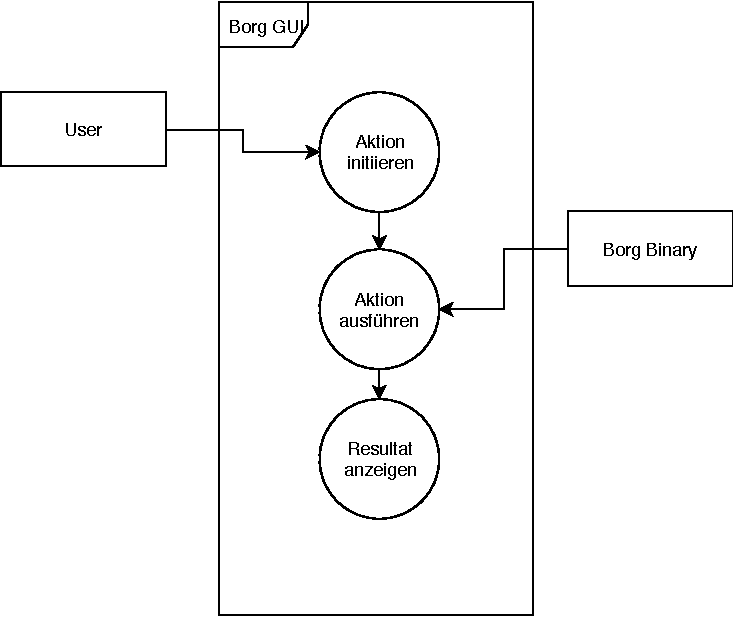
\includegraphics[width=.9\linewidth]{pictures/kontextdiagramm.pdf}
\caption{\label{fig:orgb541c49}
Kontextdiagramm des Borg GUI}
\end{figure}

\subsection{Projektmethode}
\label{sec:org29ccf63}

Für das Projekt wurde die Wasserfall-methode gewählt. Da nur eine
einzige Person am Projekt arbeitet kann nur ein Task nach dem anderen
abgearbeitet werden und viele Aufgaben stehen in Abhängigkeiten zu einander.
Somit macht das iterative Vorgehen der Wassfall-methode für dieses Projekt am
meisten Sinn.

\subsection{Konfigurationsmanagement}
\label{sec:org83f888b}

In der nachfolgenden Sektion wird definiert wie die Software und Dokumentation
versioniert wird und welche allgemeinen Werkzeuge eingesetzt werden.

\subsubsection{Versionskontrolle}
\label{sec:orgc10149d}

Die komplette Dokumentation, der Quellcode der Applikation sowie jeglich
zusäzliche Dokumente wie etwa die Zeitplanung werden mittels der Software Git
Versioniert. Thematisch zusammengehörende Änderungen werden in einem Commit
zusammengefasst. Somit ist jederzeit nachvollziehbar was wann geändert hat. Ein
Commit sollte dabei gemäss dem Artikel von Chris Beams "`How to write a Git
Commit Message"' \footcite{commit} und in englischer Sprache geschrieben sein.

Versionsnummern sind für die Applikation zum jetzigen Zeitpunkt noch nicht
vorgesehen. Sollten sie zukünftig einmal verwendet werden soll eine semantische
Versionierung \footcite{semver} verwendet. Dabei ist eine Versionsnummer immer
nach diesem Schema aufgebaut, MAJOR.MINOR.PATCH. Bei Änderungen wir die:
\begin{enumerate}
\item MAJOR Version erhöt wenn man inkompatible Änderungen an der \gls{api} macht.
\item MINOR Version erhöt wenn man Funktionalität hinzufügt die
rückwärtskompatibel ist.
\item PATCH Version erhöt wenn man rückwärtskompatible Bug-Fixes hinzufügt.
\end{enumerate}

Auf jeden Fall sollte wenn möglich immer nur lauffähiger Code im Master Branch
eingecheckt sein damit der Master Branch immer eine funktionierende Software
repräsentiert. Dies gilt auch für das Repository der Dokumentation. Der Master
Branch der Dokumentation sollte maximal mit zwei Befehlen \texttt{make clean} und
\texttt{make} "`kompilierbar "' sein.

Als Software für die Versionskontrolle wurde Git \footcite{git} aus folgenden
Gründen ausgewählt:

\begin{itemize}
\item Ist der de facto Standard bei Versionskontrollsoftware
\item Läuft auf allen gängigen Betriebssystemen
\item Es gäbe gratis Services die man nutzen könnte (Github, Gitlab)
\item Man kann offline arbeiten und Commits erstellen
\item Der Author hat bereits einen eigenen Git Server zur Verfügung
\item Der Author ist bereits mit Git aus vorhergehenden Projekten vertraut,
dadurch muss man keine Ressourcen aufwenden eine neue Software zu lernen.
Zusätzlich hat sich Git in den vorhergehenden Projekten als robuste
und schnelle Software erwiesen.
\item Git ist \gls{libre} unter der \gls{gpl} v2.
\end{itemize}

\subsubsection{Editor}
\label{sec:org9f4c43a}

Sowohl bei der Dokumentation wie auch bei der Programmierung wurde
hauptsächlich der Editor GNU Emacs \footcite{emacs} verwendet. GNU Emacs ist mit
32 Jahren (obwohl seine Wurzeln bis ins Jahre 1976 zurückgehen) wohl eines der
ältesten noch aktiven Software Projekte. Emacs ist \gls{libre} unter der
\gls{gpl} v3. Emacs wurde gewählt da es ein schneller, schlanker und sehr
flexibler Texteditior ist. Von normaler Textmanipulation über Taskmanagement
und Emails schreiben ist alles möglich.

\subsubsection{Dokumentation}
\label{sec:orgf78de20}

Diese Dokumentation wurde in Org-mode \footcite{orgmode}, einer Erweiterung für
den Text Editor Emacs, geschrieben. Die Syntax erinnert an Markdown und
Org-mode bietet einem eine vielzahl an Hilfen dafür inklusive dem erstellen von
Tabellen und Spreadsheet Funktionen. Für finalle Version des Dokuments kann
Org-mode die ursprünglich Textdatei über \LaTeX{} in ein PDF exportieren.

\LaTeX{} \footcite{latex} ist eine Software, welche einem die Benutzung des
Textsatzsystems TeXs vereinfacht. \LaTeX{} wurde gegenüber einem "`What You See Is
What You Get"' (z.Bsp. MS. Word), Editor gewählt weil es einem mit seiner Markup
Sprache erlaubt das Dokument in Text Dateien zu erstellen, gerade für
Programmiere ist dies eine sehr interessante Lösung. Dadurch, dass \LaTeX{} auch
nur aus reinen Textdateien besteht, kann man die Dokumente auch ohne weiteres
in die Versionskontrollsoftware einchecken und die Entwicklung im Log
zurückverfolgen. \LaTeX{} ist \gls{libre} unter der \LaTeX{} Project Public
License.

Die Grafiken in diesem Dokument wurden hauptsächlich mit dem Vektor Grafik
Editor Inkscape \footcite{inkscape} erstellt. Inkscape ist \gls{libre} unter der
GNU Public License v3.

Die Diagramme wurden mit Draw.io \footcite{draw} erstellt. Draw.io ist \gls{libre}
unter Apache Lizenz Version 2.0 \footcite{apache} und kann sowohl als Desktop
Applikation wie auch als Webanwendung genutzt werden.

Beim Design der Arbeit wurden soweit als möglich die typgraphischen Regeln aus
dem Buch "`Practical Typography"' von Matthew Butterick \footcite{typo} angewandt.
Bei den Diagrammen wurden aussschliesslich Farben aus der von Google
entwickelten Design Sprache "`Material"'\footcite{material} eingesetzt.

\subsection{Zeitplanung}
\label{sec:orgd7e5234}

Die detaillierte Zeitplanung ist dem Ganttchart in der Datei
\href{Zeitplanung\_Andreas\_Zweili.html}{Zeitplanung\_Andreas\_Zweili.html} zu entnehmen. Bei der Zeitplanung wurde darauf
geachtet das die Arbeit soweit als möglich nicht mit dem Berufsleben kolidiert.
An einem normalen Arbeitstag wurde dabei damit gerechnet das ca. 2 Stunden
Arbeit am Abend möglich sein sollten. An einem arbeitsfreien Tag wurde mit 6
Stunden arbeit gerechnet. Über die Festtage wurden diverse Tage von der Planung
ausgenommen da es nicht realistisch schien das an diesen Tagen die Arbeit
signifikant vorwärts gehen würde. Auch Schultage wurde nicht als Arbeitstage
gerechnet da man meist nicht mehr für weitere Tätigkeiten gross motiviert ist.

Als zusätliche Massnahme um die Arbeitslast zu verteilen wurde vom 14. Januar
bis zum 11. März jeder Montag auf der Arbeitsstelle als frei eingegeben.
Dadurch steht wärend des Projektes etwas mehr Zeit zur verfügung als sonst mit
einer 100\% Arbeitsstelle möglich wäre.

\subsection{Controlling}
\label{sec:orgc9e0677}

Das Controlling wird verwendet um zu kontrollieren das die eigentliche Planung
mit dem effektiv geleisteten Aufwand respektive den effektiv verwendeten
Ressourcen übereinstimmt. Somit können für zukünftige Projekte Lehren gezogen
werden.

\newpage
\begin{landscape}
\subsubsection{Zeit}
\label{sec:org49761cd}

\begin{longtable}{|p{3cm}|p{5cm}|p{3cm}|p{7cm}|}
\hline
\textbf{Aufgabe}\cellcolor[HTML]{C0C0C0} & \textbf{Gesch. Aufwand}\cellcolor[HTML]{C0C0C0} & \textbf{Effekt. Aufwand}\cellcolor[HTML]{C0C0C0} & \textbf{Begründung}\cellcolor[HTML]{C0C0C0}\\
\hline
\endfirsthead
\multicolumn{4}{l}{Fortsetzung von vorheriger Seite} \\
\hline

\textbf{Aufgabe}\cellcolor[HTML]{C0C0C0} & \textbf{Gesch. Aufwand}\cellcolor[HTML]{C0C0C0} & \textbf{Effekt. Aufwand}\cellcolor[HTML]{C0C0C0} & \textbf{Begründung}\cellcolor[HTML]{C0C0C0} \\

\hline
\endhead
\hline\multicolumn{4}{r}{Fortsetzung nächste Seite} \\
\endfoot
\endlastfoot
\hline
\hline
 & \textbf{Gesamter Aufwand} &  & \\
\hline
\caption{\label{tab:orga70bdbf}
Zeitcontrolling}
\\
\end{longtable}

\newpage
\subsubsection{Ressourcen}
\label{sec:orge70a0d3}

Folgende Ressourcen werden wärend der Arbeit benötigt:
\begin{longtable}{|p{5cm}|p{3cm}|p{3cm}|p{7cm}|}
\hline
\textbf{Ressource}\cellcolor[HTML]{C0C0C0} & \textbf{geschätzte Stück}\cellcolor[HTML]{C0C0C0} & \textbf{effekt. Stück}\cellcolor[HTML]{C0C0C0} & \textbf{Begründung}\cellcolor[HTML]{C0C0C0}\\
\hline
\endfirsthead
\multicolumn{4}{l}{Fortsetzung von vorheriger Seite} \\
\hline

\textbf{Ressource}\cellcolor[HTML]{C0C0C0} & \textbf{geschätzte Stück}\cellcolor[HTML]{C0C0C0} & \textbf{effekt. Stück}\cellcolor[HTML]{C0C0C0} & \textbf{Begründung}\cellcolor[HTML]{C0C0C0} \\

\hline
\endhead
\hline\multicolumn{4}{r}{Fortsetzung nächste Seite} \\
\endfoot
\endlastfoot
\hline
Projektleiter/Mitarbeiter & 1 & 1 & \\
Diplombetreuer & 1 & 1 & \\
Testuser & 5 &  & \\
Korrekturleser & 3 &  & \\
iPad & 1 & 1 & \\
Notebook & 1 & 1 & \\
\hline
\caption{\label{tab:orge203351}
Ressourcen}
\\
\end{longtable}
\end{landscape}

\subsubsection{Kosten}
\label{sec:org4c0ace3}

Werden die internen Lohnkosten des Projektleiters auf ca. 60 CHF pro Stunde
geschätzt ergeben sich aus der Zeitplanung somit theoretische Kosten von 19'200
CHF für die Umsetzung dieser Arbeit. Da dieses Projekt finanziell jedoch in
keinster Weise wirtschaftliche relevant ist, sind die Kosten nur ein rein
theoretischer Faktor.
\begin{table}[htbp]
\centering
\begin{tabular}{lrr}
\hline
\textbf{Name}\cellcolor[HTML]{C0C0C0} & \textbf{Aufwand in h}\cellcolor[HTML]{C0C0C0} & \textbf{Kosten in CHF}\cellcolor[HTML]{C0C0C0}\\
\hline
Initialisierung & 24 & 1440\\
Analyse & 47 & 2820\\
Konzept & 34 & 2040\\
Realisierung & 172 & 10320\\
Ausblick & 8 & 480\\
Arbeit korrigieren & 20 & 1200\\
Meeting \#1 & 5 & 300\\
Meeting \#2 & 5 & 300\\
Meeting \#3 & 5 & 300\\
\hline
\textbf{Total} & 320 & 19200\\
\hline
\end{tabular}
\caption{\label{tab:org6829dd7}
Kostenrechnung}

\end{table}

\subsection{Projektrisiken}
\label{sec:org51109de}

Das Risikomanagement dient dazu Risiken im Projekt zu erkennen und Massnahmen
zur Vermeidung der Risiken zu definieren. Dadurch steht man ihnen nicht
unvorbereitet gegenüber sollten sie eintreffen.

\subsubsection{Risikobeschreibung}
\label{sec:org3b92534}

In der Tabelle: (\ref{tab:org606c2c8}), sind die Risiken des Projektes
gemeinsam mit ihren Gegenmassnahmen aufgelistet. Jedes Risiko wurde
entsprechend der Tabelle: (\ref{tab:org826ea60}) nach der Wahrscheinlichkeit
des Eintreffens bewertet und entsprechend der Tabelle: (\ref{tab:orgee0e694}) nach
seiner Auswirkung bewertet.

\begin{longtable}{|p{0.45\textwidth}|p{0.45\textwidth}|}
\hline
\textbf{Beschreibung}\cellcolor[HTML]{C0C0C0} & \textbf{Massnahmen}\cellcolor[HTML]{C0C0C0}\\
\hline
\endfirsthead
\multicolumn{2}{l}{Fortsetzung von vorheriger Seite} \\
\hline

\textbf{Beschreibung}\cellcolor[HTML]{C0C0C0} & \textbf{Massnahmen}\cellcolor[HTML]{C0C0C0} \\

\hline
\endhead
\hline\multicolumn{2}{r}{Fortsetzung nächste Seite} \\
\endfoot
\endlastfoot
\hline
Ein grösseres Problem in der Programmierung blockiert den Fortschritt. & Immer nur eine Sache auf einmal in der Code-Basis ändern, alle Fehler beheben und erst dann zur nächsten Aufgabe weitergehen.\\
\hline
Viel Arbeit an der Arbeitsstelle, dabei bleibt weniger Zeit für die Diplomarbeit. & Auf der Arbeit Freitage eingeben um die Last etwas zu verteilen. Projektplanung machen.\\
\hline
Know-How zur Umsetzung ist nicht vollständig vorhanden. & Gute Informationsbeschaffung im Internet, Büchern, etc.\\
\hline
Manuelle Tests brauchen zu viel Zeit. & Soviel wie möglich automatisieren. Dabei jedoch nicht den Fokus auf die eigentliche Entwicklung verlieren.\\
\hline
Die Programmierung des Programms benötigt zu viel Zeit. & Bei der Projektplanung genau definieren was die GUI Applikation beinhalten muss. Ziele definieren, Abgrenzungen treffen.\\
\hline
User haben keine Zeit für Utility Tests. & Vorgängig einen Termin abmachen.\\
\hline
\gls{borg} ändert fundamental seine \gls{api}. & Gegen eine fixe Version von \gls{borg} entwickeln.\\
\hline
\caption{\label{tab:orgdbf2ea4}
Projektrisiken}
\\
\end{longtable}

\section{Analyse}
\label{sec:org69ba381}
\subsection{Umweltanalyse}
\label{sec:org0b1a0ff}

Die Projektumwelt-Analyse ist eine Methode, die Beziehungen,
Erwartungshaltungen und Einflüsse auf das Projekt durch interne und
externe soziale Umwelten zu betrachten und zu bewerten. Auf Grundlage
der Analyseergebnisse werden erforderliche Massnahmen zur Gestaltung
der Umweltbeziehungen abgeleitet. Die Gestaltung der
Projektumweltbeziehungen ist eine Projektmanagementaufgabe. In der
Tabelle:(\ref{tab:orgd4b119b}) wurden die Anforderungen und Wünsche
mit Einschätzung der Wahrscheinlichkeit und der Einflussnahme aufgenommen.
Zusätzlich ist die Beziehung der Stakeholder zum Projekt noch in der
Abbildung:(\ref{fig:org5fa0b49}) grafisch dargestellt.

Da das Projekt so ausgelegt ist das der Projektleiter es in Eigenarbeit
verwirklichen kann ist der Einfluss der Stakeholder wärend der Umsetzung sehr
gering. Die User werden bei der Entwicklung mittels einer "`Usability"' Studie
miteinbezogen und die \gls{borg} Community wird mit regelmässigen Posts auf dem
offiziellen Github Repository auf dem Laufenden gehalten.
Nach Ende der Diplomarbeit soll das Projekt für interessierte Entwickler jedoch
offen sein. Der Quellcode wird bereits während der Arbeit öffentlich zur
Verfügung gestellt.

\begin{figure}[htbp]
\centering
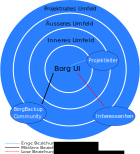
\includegraphics[width=.9\textwidth]{pictures/stakeholder_diagramm.pdf}
\caption{\label{fig:org5fa0b49}
Stakeholder Diagramm}
\end{figure}

\newpage
\begin{landscape}
\begin{table}[htbp]
\centering
\begin{tabular}{|>{\columncolor[HTML]{EFEFEF}}p{0.8cm}|l|l|p{8cm}|l|}
\hline
\textbf{Nr}.\cellcolor[HTML]{C0C0C0} & \textbf{Stakeholder}\cellcolor[HTML]{C0C0C0} & \textbf{Einfluss}\cellcolor[HTML]{C0C0C0} & \textbf{Anforderung/Wünsche}\cellcolor[HTML]{C0C0C0} & \textbf{Wahrscheinlichkeit}\cellcolor[HTML]{C0C0C0}\\
\hline
1. & BorgBackup Community & gering & - Eine Applikation die den Umfang von BorgBackup abdeckt & mittel\\
 &  &  & - Open-Source & hoch\\
 &  &  & - Mitsprachrecht bei der Entwicklung & niedrig\\
\hline
2. & User & gering & - Eine einfache Anwendung & hoch\\
 &  &  & - Einmal einrichten und vergessen & mittel\\
\hline
3. & Interessenten & gering & - Einfach verständliches Projekt Repository & hoch\\
 &  &  & - Einfaches Setup zum testen & hoch\\
\hline
4. & Projektleiter & hoch & - Stabile Anwendung erstellen & mittel\\
 &  &  & - Ein nachhaltiges Projekt starten & mittel\\
 &  &  & - Anerkennung im fachlichen Umfeld & hoch\\
\hline
\end{tabular}
\caption{\label{tab:orgd4b119b}
Umwelt-Analyse}

\end{table}
\end{landscape}

\subsection{Risiko-Analyse}
\label{sec:org6fcac9b}

Bei der Risikoanalyse wird von einem durchschnittlichen Benutzer ausgegangen
der zur Zeit noch keine Backups macht und beginnen möchte \gls{borg} zu nutzen um
auf einer externen Harddisk seine Backups zu speichern.

Es wird dabei eine Ist/Soll Analyse gemacht um die Lösung gegenüber der
bestehenden Möglichkeiten zu vergleichen. Jedes Risiko wurde entsprechend der
Tabelle: (\ref{tab:org826ea60}) nach der Wahrscheinlichkeit des Eintreffens
bewertet und entsprechend der Tabelle: (\ref{tab:orgee0e694}) nach seiner Auswirkung
im Bezug auf die Nützlichkeit der gemachten Backups.

In der Tabelle: (\ref{tab:org606c2c8}) sind dabei die Risiken für das
Szenario aufgelistet und nummeriert. In der, Abbildung:(\ref{fig:org85added}), ist die
Bewertung des Ist-Risikos grafisch dargestellt und in der,
Abbildung:(\ref{fig:org5e0b50f}), ist das Soll-Risiko welches mit dieser Arbeit
angestrebt wird ebenfalls grafisch dargestellt.

Es sollte im Rahmen der Arbeit möglich sein die meisten Risiken zu verringern.
Da automatische Hintergrundbackups jedoch nur ein Kann-Ziel sind wir in dieser
Analyse nicht davon ausgegangen das man das Risiko Nr. 5 im Rahmen dieser
Arbeit reduzieren kann.

\begin{table}[H]
\centering
\begin{tabular}{l|l}
\textbf{Bewertung} & \textbf{Beschreibung: Wahrscheinlichkeit (W)}\\
\hline
1 = gering & Unwahrscheinlich, <20\%\\
2 = mittel & Mässig wahrscheinlich, 20-50\%\\
3 = hoch & Hohe Wahrscheinlichkeit > 50\%\\
\end{tabular}
\caption{\label{tab:org826ea60}
Risikobewertung Wahrscheinlichkeit}

\end{table}

\begin{table}[H]
\centering
\begin{tabular}{l|l}
\textbf{Bewertung} & \textbf{Beschreibung: Auswirkung (A)}\\
\hline
1 = gering & Geringe Auswirkungen auf Nützlichkeit\\
2 = mittel & Mittlere Auswirkung auf die Nützlichkeit\\
3 = hoch & Hohe Auswirkung auf die Nützlichkeit\\
\end{tabular}
\caption{\label{tab:orgee0e694}
Risikobewertung Auswirkung}

\end{table}

\begin{table}[H]
\centering
\begin{tabular}{|>{\columncolor[HTML]{EFEFEF}}p{0.1\textwidth}|p{0.8\textwidth}|}
\hline
\textbf{Nr.}\cellcolor[HTML]{C0C0C0} & \textbf{Beschreibung}\cellcolor[HTML]{C0C0C0}\\
\hline
1. & Der Benutzer hat noch nie die Kommandozeile verwendet und scheitert bereits an der Installation von \gls{borg}.\\
\hline
2. & Der Benutzer verwendet keine Verschlüsselung und verliert seine Harddisk.\\
\hline
3. & Der Benutzer speichert die Backups auf der internen statt der externen Harddisk.\\
\hline
4. & Der Benutzer löscht aus Versehen ein Backup.\\
\hline
5. & Der Anwender vergisst die Backups zu machen.\\
\hline
\end{tabular}
\caption{\label{tab:org606c2c8}
Risikobeschreibung}

\end{table}

\begin{figure}[H]
\centering
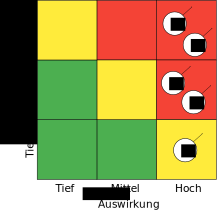
\includegraphics[width=9cm]{pictures/istrisiko.pdf}
\caption{\label{fig:org85added}
Grafische Darstellung der Ist-Risikoanalyse}
\end{figure}

\begin{figure}[H]
\centering
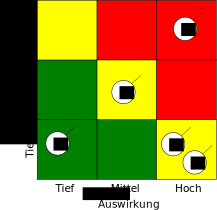
\includegraphics[width=9cm]{pictures/sollrisiko.pdf}
\caption{\label{fig:org5e0b50f}
Grafische Darstellung der Soll-Risikoanalyse}
\end{figure}

\newpage
\subsection{SWOT-Analyse}
\label{sec:orgd45af75}

Die SWOT-Analyse ist eine Methode, die Stärken, Schwächen, Chancen und
Gefahren zu erkennen, indem eine 4-Felder-Matrix ausgefüllt wird.

Wichtig vor dem Ausfüllen der SWOT-Analyse ist es, ein klares Ziel zu
haben. Die ausgefüllte SWOT-Analyse für dieses Projekt ist in der
Abbildung:(\ref{fig:org5fafa63}) zu sehen.

\begin{figure}[htbp]
\centering
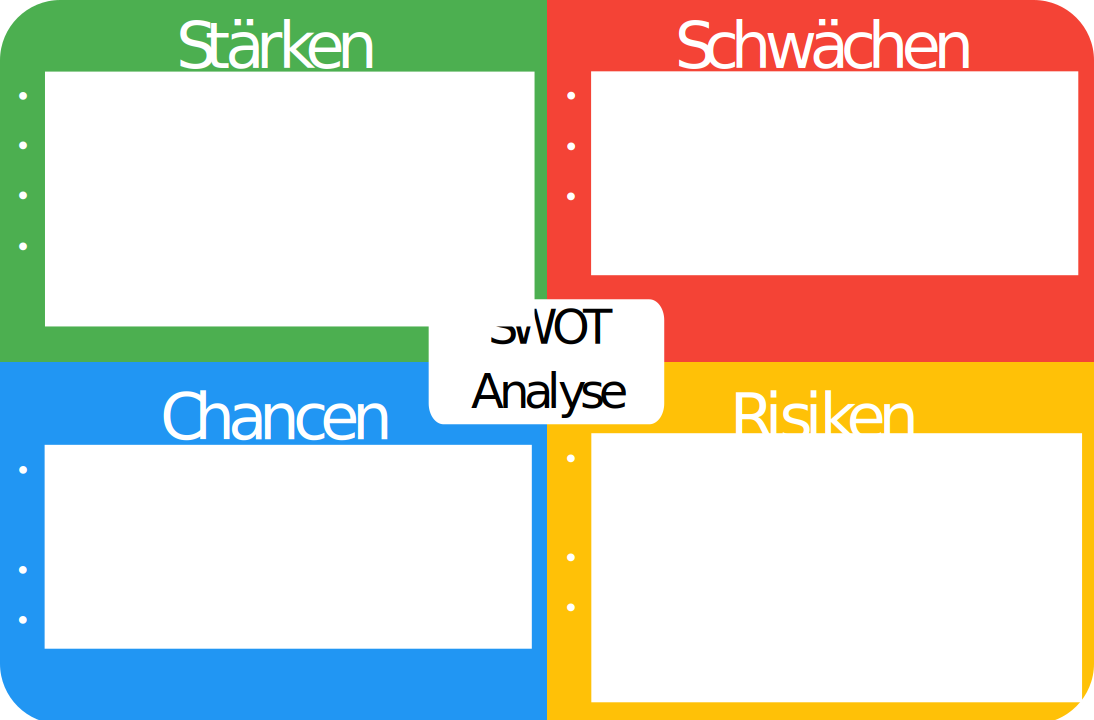
\includegraphics[width=.9\linewidth]{pictures/swot_analyse.pdf}
\caption{\label{fig:org5fafa63}
SWOT Analyse des Projektes}
\end{figure}

\subsection{Anforderungskatalog}
\label{sec:org82903aa}

Der Anforderungskatalog entspricht 1:1 den Zielen welche in der Tabelle
\ref{tab:org9275be4} definiert wurden.

\subsection{Use Cases}
\label{sec:orgc44612b}

Ein Use Case sammelt alle möglichen Szenarien, die eintreten können,
wenn ein Akteur versucht, mit Hilfe des betrachteten Systems ein
bestimmtes Ziel zu erreichen. Dabei beschreibt er, was beim Versuch der
Zielerreichung passieren kann. Je nach Ablauf kann auch ein Fehlschlag
ein Ergebnis eines Anwendungsfalls sein (e.g. falsches Passwort beim
Login). Dabei wird die technische Lösung nicht konkret beschrieben.
Die Detailstufe kann dabei sehr unterschiedlich sein.\footcite{usecase}

\subsubsection{Anwendungsfalldiagramm}
\label{sec:orge2f5022}

"`Ein Anwendungsfalldiagramm \ldots{} ist eine der 14 Diagrammarten der
Unified Modelling Language (UML), einer Sprache für die Modellierung
der Strukturen und des Verhaltens von Software- und anderen Systemen.
Es stellt Anwendungsfälle und Akteure mit ihren jeweiligen
Abhängigkeiten und Beziehungen dar."'\footcite{usecasediagramm}

Das Anwendungsfalldiagramm für das \gls{borg} \gls{gui} ist in der Abbildung:
(\ref{fig:orgc9a56f0}) zu sehen.

\newpage
\begin{landscape}
\begin{figure}[htbp]
\centering
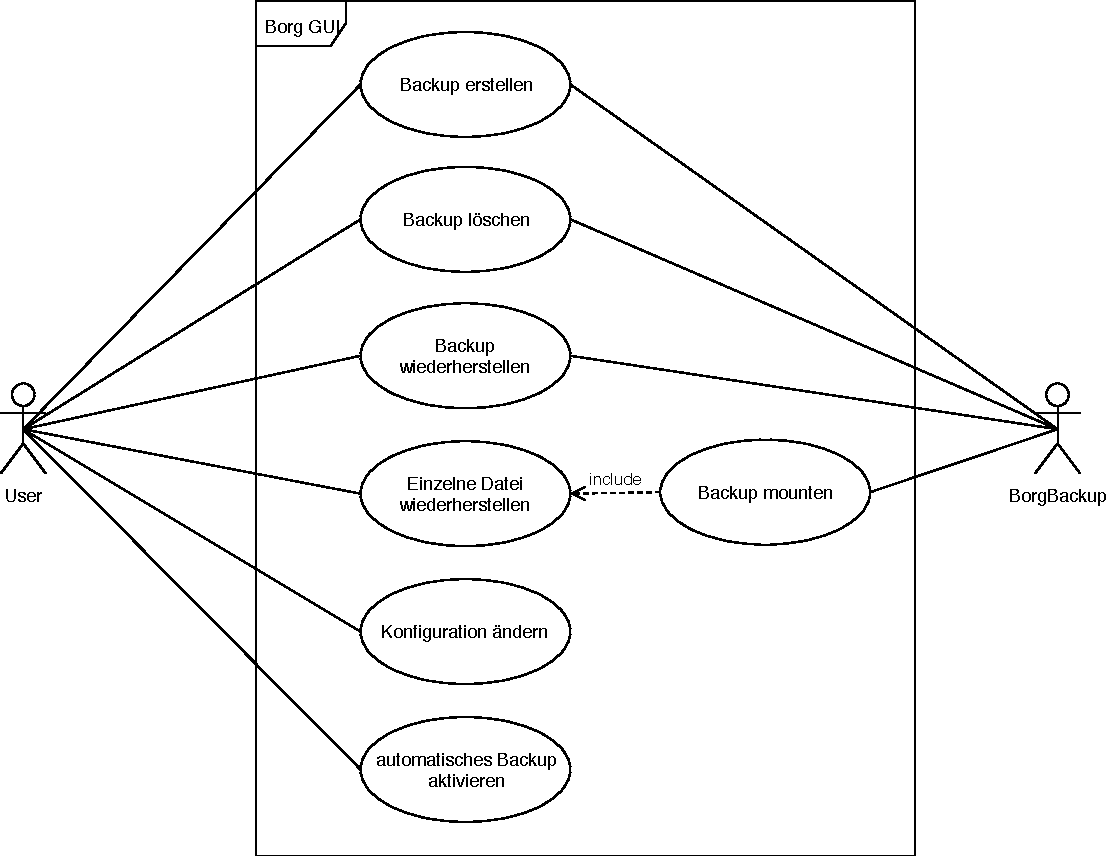
\includegraphics[width=.9\linewidth]{pictures/use_case.pdf}
\caption{\label{fig:orgc9a56f0}
Anwendungsfalldiagramm}
\end{figure}
\end{landscape}
\newpage

\subsubsection{Use Cases Detailbeschreibung}
\label{sec:org179a393}

Use Cases werden in der Regel mit Hilfe einer sogenannten Use Case Schablone im
Detail beschrieben, damit klar ist, wie der Ablauf jeweils genau aussieht. Die
in diesem Projekt verwendete Schablone wurde von Alistair Cockburn definiert.

Die nachfolgend aufgeführten Use Cases, Tabellen:(\ref{tab:org9200604}, \ref{tab:org4b98c25},
\ref{tab:org7b118df}, \ref{tab:orged9864f}, \ref{tab:orga3274db}, \ref{tab:org4ea078d}, \ref{tab:org3890696})
wurden dem Anwendungsfalldiagramm, Abbildung:(\ref{fig:orgc9a56f0}), entnommen und
zusätzlich noch um jeweils ein Aktivitätsdiagramm , Abbildungen:
(\ref{fig:org8d383e4}, \ref{fig:org96d7936}, \ref{fig:orgb1cc6ad},
\ref{fig:org992f6bb}, \ref{fig:org35467e2}, \ref{fig:org839581b}), erweitert
um den Ablauf verständlicher zu machen.

Ein Aktivitätsdiagramm ist dabei ein hilfreiches UML Diagramm zum Erweitern von
Use Cases und zeigt einem gut die Zuständigkeiten der Aktoren auf.

\paragraph{Use Case 1.0 Backup erstellen}
\label{sec:org9166a09}

{\footnotesize
\begin{longtable}{|>{\columncolor[HTML]{EFEFEF}}p{.235\textwidth}|p{.7\textwidth}|}
\hline
\textbf{Identifier + Name} & 1.0 Backup erstellen\\
\hline
\endfirsthead
\multicolumn{2}{l}{Fortsetzung von vorheriger Seite} \\
\hline

\textbf{Identifier + Name} & 1.0 Backup erstellen \\

\hline
\endhead
\hline\multicolumn{2}{r}{Fortsetzung nächste Seite} \\
\endfoot
\endlastfoot
\hline
\textbf{Description} & Das erstellen einer Datensicherung durch \gls{borg} anstossen.\\
\hline
\textbf{Actors} & Benutzer\\
\hline
\textbf{Status} & Freigegeben\\
\hline
\textbf{Includes} & -\\
\hline
\textbf{Trigger} & User möchte ein Backup erstellen.\\
\hline
\textbf{Preconditions} & Die Applikation wurde gestartet.\\
\hline
\textbf{Postconditions} & Das erstellte Backup wird angezeigt.\\
\hline
\textbf{Normal Flow} & 1. Den Quellpfad auswählen.\\
 & 2. Den Button "`Backup"' anklicken.\\
 & 3. Ein Pop mit Fortschrittsbalken erscheint und zeigt die Zeit bis zum Ende des Backups an.\\
 & 4. Am Ende des Backups verschwindet das Pop-up wieder.\\
 & 5. Die Liste der Backups aktualisiert sich.\\
\hline
\textbf{Alternative Flow} & -\\
\hline
\textbf{Notes} & -\\
\hline
\textbf{UC History} & 1.0 Draft erstellt durch AZ\\
\hline
\textbf{Author} & A. Zweili\\
\hline
\textbf{Date} & 30.12.2018\\
\hline
\caption{\label{tab:org9200604}
Use Case 1.0 Backup erstellen}
\\
\end{longtable}
}
\begin{figure}[htbp]
\centering
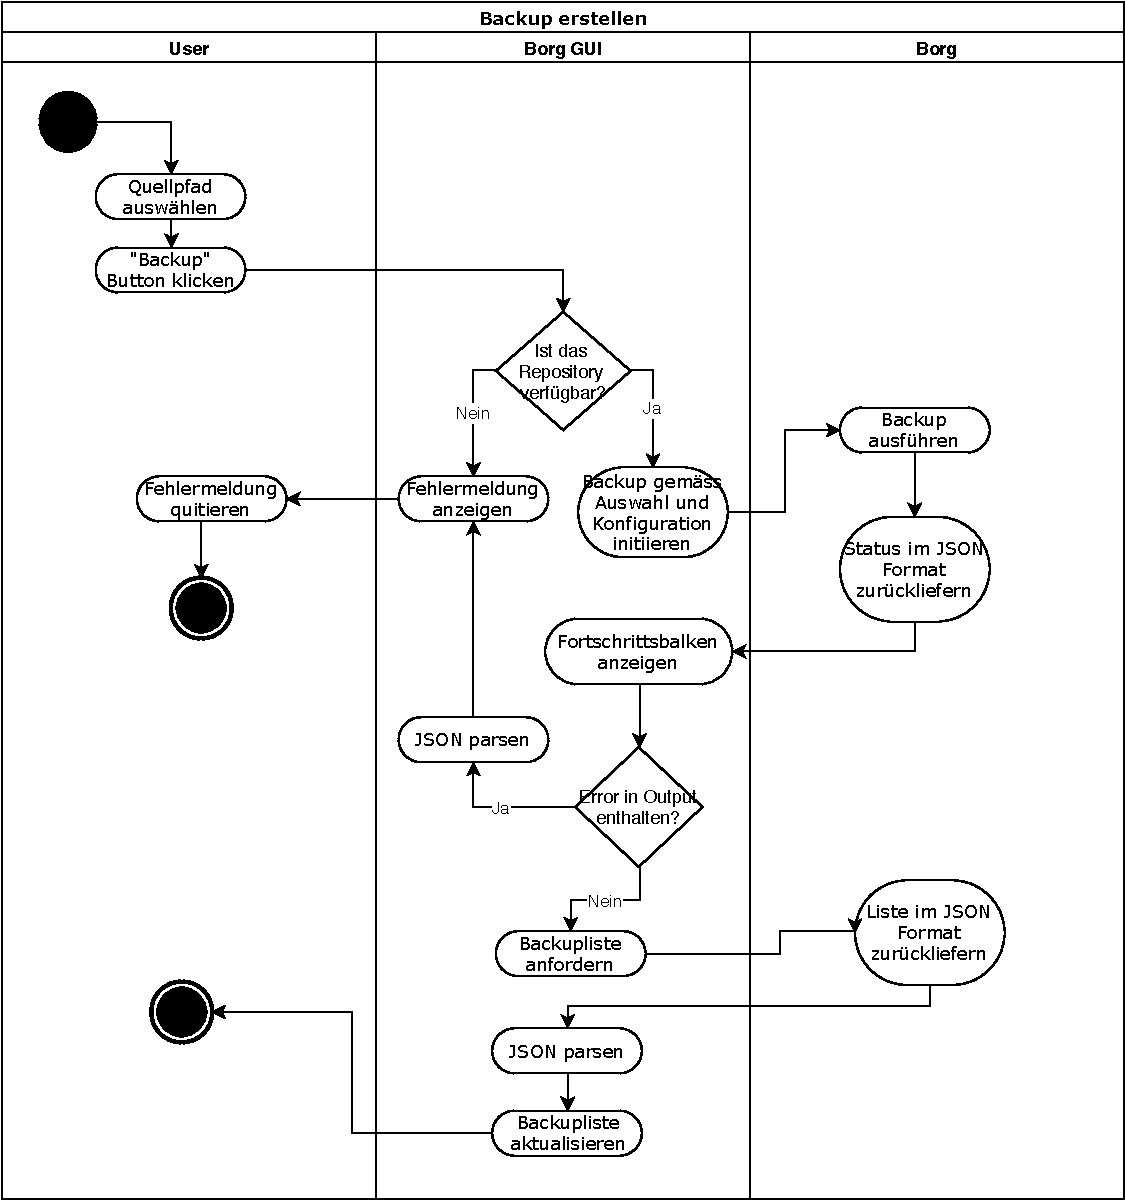
\includegraphics[width=.9\linewidth]{pictures/activity_backup.pdf}
\caption{\label{fig:org8d383e4}
Aktivitätsdiagramm zum Erstellen eines Backups}
\end{figure}
\newpage
\paragraph{Use Case 2.0 Backup löschen}
\label{sec:orga845097}

{\footnotesize
\begin{longtable}{|>{\columncolor[HTML]{EFEFEF}}p{.235\textwidth}|p{.7\textwidth}|}
\hline
\textbf{Identifier + Name} & 2.0 Backup löschen\\
\hline
\endfirsthead
\multicolumn{2}{l}{Fortsetzung von vorheriger Seite} \\
\hline

\textbf{Identifier + Name} & 2.0 Backup löschen \\

\hline
\endhead
\hline\multicolumn{2}{r}{Fortsetzung nächste Seite} \\
\endfoot
\endlastfoot
\hline
\textbf{Description} & Ein zuvor erstelltes Backup wird gelöscht.\\
\hline
\textbf{Actors} & Benutzer\\
\hline
\textbf{Status} & Freigegeben\\
\hline
\textbf{Includes} & -\\
\hline
\textbf{Trigger} & Ein User möchte ein bestehendes Backup löschen.\\
\hline
\textbf{Preconditions} & Use Case 1.0 ausgeführt.\\
\hline
\textbf{Postconditions} & Das gelöschte Backup wird nicht mehr aufgelistet.\\
\hline
\textbf{Normal Flow} & 1. Ein Backup aus der Liste auswählen.\\
 & 2. Den Button "`Delete anklicken"'.\\
 & 3. Ein Bestätigungsdialog erscheint.\\
 & 4. Im Dialog den "`Ok"' Button anklicken.\\
\hline
\textbf{Alternative Flow} & 1. Ein Backup aus der Liste auswählen.\\
 & 2. Den Button "`Delete anklicken"'.\\
 & 3. Ein Bestätigungsdialog erscheint.\\
 & 4. Die Aktion mit einem Klick auf den "`Cancel"' Button abbrechen.\\
\hline
\textbf{Notes} & -\\
\hline
\textbf{UC History} & 1.0 Draft erstellt durch AZ\\
\hline
\textbf{Author} & A. Zweili\\
\hline
\textbf{Date} & 30.12.2018\\
\hline
\caption{\label{tab:org4b98c25}
Use Case 2.0 Backup löschen}
\\
\end{longtable}
}
\begin{figure}[htbp]
\centering
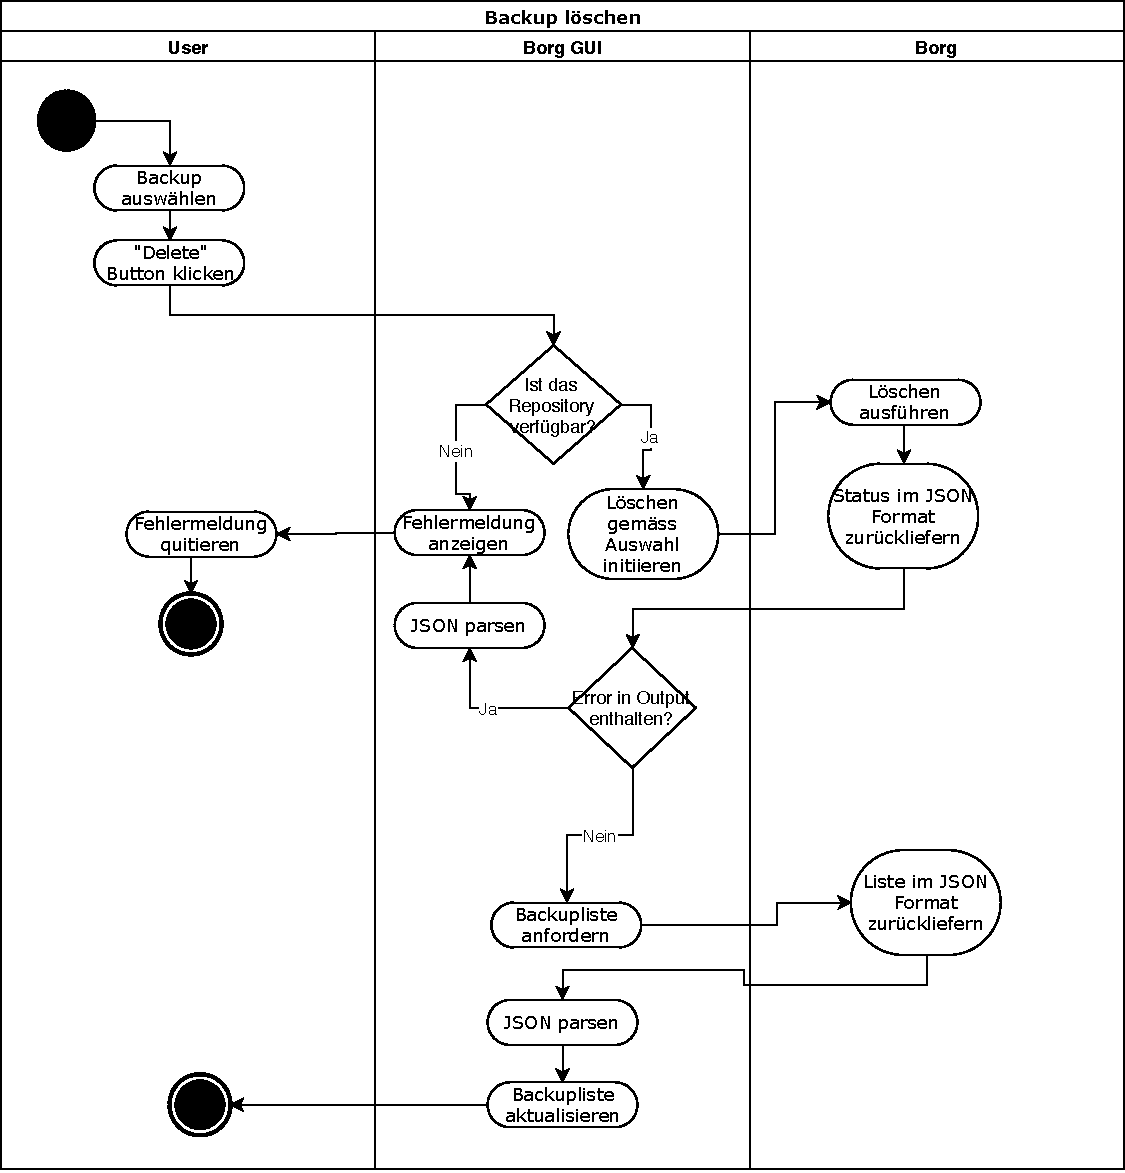
\includegraphics[width=.9\linewidth]{pictures/activity_delete.pdf}
\caption{\label{fig:org96d7936}
Aktivitätsdiagramm zum Löschen eines Backups}
\end{figure}
\newpage
\paragraph{Use Case 3.0 Backup wiederherstellen}
\label{sec:orgb1c5081}

{\footnotesize
\begin{longtable}{|>{\columncolor[HTML]{EFEFEF}}p{.235\textwidth}|p{.7\textwidth}|}
\hline
\textbf{Identifier + Name} & 3.0 Backup wiederherstellen\\
\hline
\endfirsthead
\multicolumn{2}{l}{Fortsetzung von vorheriger Seite} \\
\hline

\textbf{Identifier + Name} & 3.0 Backup wiederherstellen \\

\hline
\endhead
\hline\multicolumn{2}{r}{Fortsetzung nächste Seite} \\
\endfoot
\endlastfoot
\hline
\textbf{Description} & Alle Dateien eines Backups wiederherstellen.\\
\hline
\textbf{Actors} & User\\
\hline
\textbf{Status} & Freigegeben\\
\hline
\textbf{Includes} & -\\
\hline
\textbf{Trigger} & Daten sollen wieder hergestellt werden.\\
\hline
\textbf{Preconditions} & Use Case 1.0 wurde ausgeführt.\\
\hline
\textbf{Postconditions} & Die Dateien aus dem Backup wurde im angegeben Pfad wiederhergestellt.\\
\hline
\textbf{Normal Flow} & 1. Ein Backup aus der Liste auswählen.\\
 & 2. Den Button "`Restore"' klicken.\\
 & 3. Ein Pop-Up zur Auswahl eines Zielpfades erscheint.\\
 & 4. Den Zielpfad mit klick auf "`Choose"' bestätigen.\\
 & 5. Ein Dateiexplorer öffnet sich mit dem ausgewählt Pfad und enthält die Dateien aus dem Backup.\\
\hline
\textbf{Alternative Flow} & 1. Ein Backup aus der Liste auswählen.\\
 & 2. Den Button "`Restore"' klicken.\\
 & 3. Ein Pop-Up zur Auswahl eines Zielpfades erscheint.\\
 & 4. Die Aktion mit klick auf "`Cancel"' abbrechen.\\
\hline
\textbf{Notes} & -\\
\hline
\textbf{UC History} & 1.0 Draft erstellt durch AZ\\
\hline
\textbf{Author} & A. Zweili\\
\hline
\textbf{Date} & 30.12.2018\\
\hline
\caption{\label{tab:org7b118df}
Use Case 3.0 Backup wiederherstellen}
\\
\end{longtable}
}

\begin{figure}[htbp]
\centering
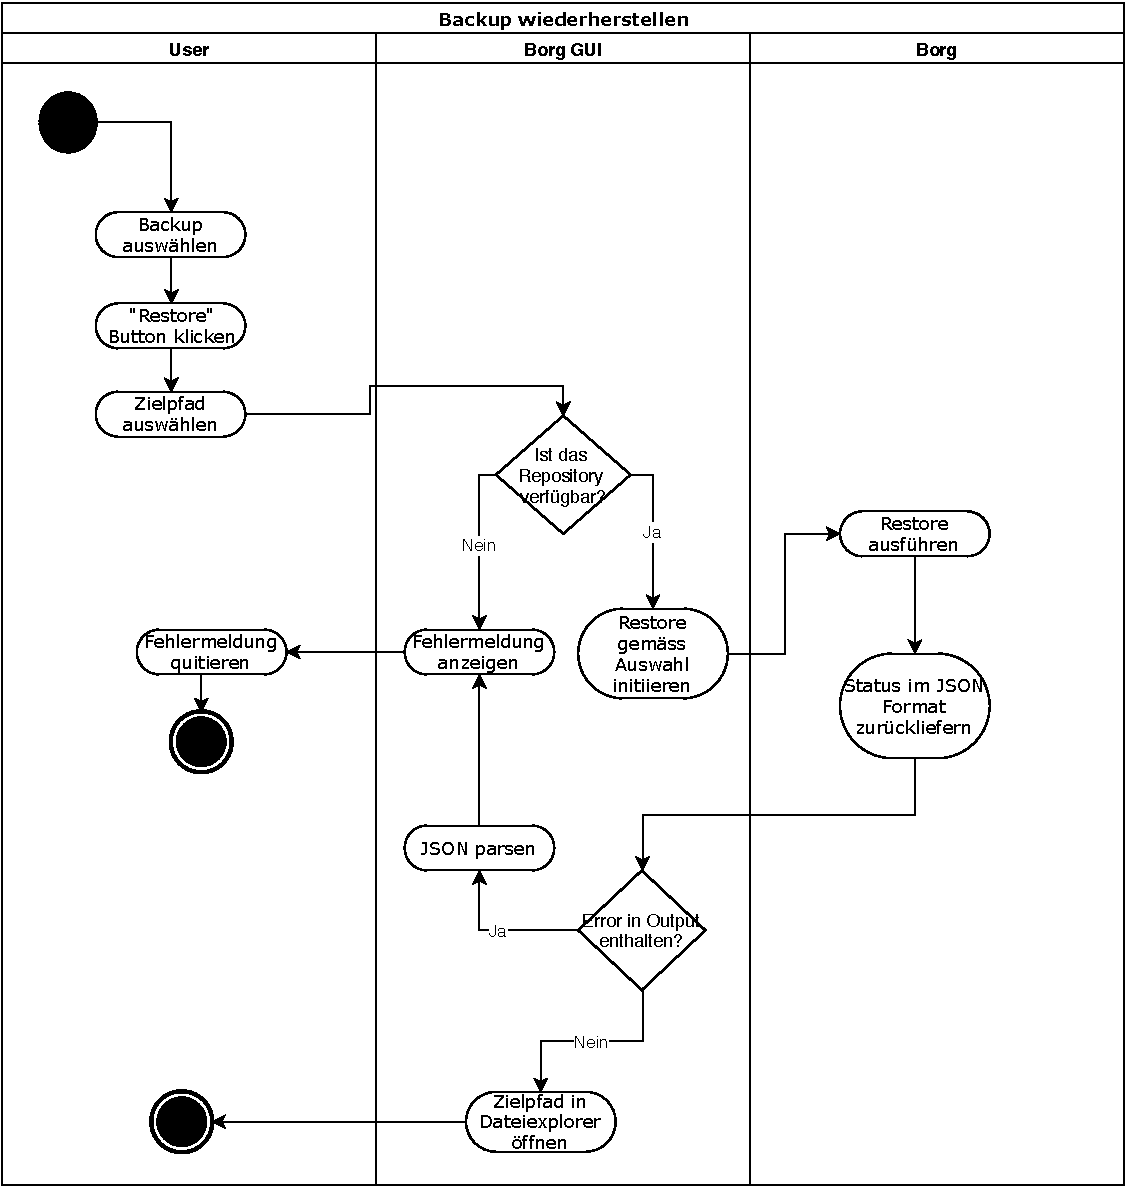
\includegraphics[width=.9\linewidth]{pictures/activity_restore.pdf}
\caption{\label{fig:orgb1cc6ad}
Aktivitätsdiagramm zum Wiederherstellen eines Backups}
\end{figure}
\newpage
\paragraph{Use Case 4.0 Einzelne Datei wiederherstellen}
\label{sec:org8e173a3}

{\footnotesize
\begin{longtable}{|>{\columncolor[HTML]{EFEFEF}}p{.235\textwidth}|p{.7\textwidth}|}
\hline
\textbf{Identifier + Name} & 4.0 Einzelne Datei wiederherstellen\\
\hline
\endfirsthead
\multicolumn{2}{l}{Fortsetzung von vorheriger Seite} \\
\hline

\textbf{Identifier + Name} & 4.0 Einzelne Datei wiederherstellen \\

\hline
\endhead
\hline\multicolumn{2}{r}{Fortsetzung nächste Seite} \\
\endfoot
\endlastfoot
\hline
\textbf{Description} & Das spezifische Wiederherstellen von einer oder mehreren Dateien.\\
\hline
\textbf{Actors} & User\\
\hline
\textbf{Status} & Freigegeben\\
\hline
\textbf{Includes} & Use Case 4.1\\
\hline
\textbf{Trigger} & Daten sollen wieder hergestellt werden.\\
\hline
\textbf{Preconditions} & Use Case 1.0 wurde ausgeführt.\\
\hline
\textbf{Postconditions} & -\\
\hline
\textbf{Normal Flow} & 1. Ein Backup aus der Liste auswählen.\\
 & 2. Auf den Button "`Mount"' klicken.\\
 & 3. Use Case 4.1 wird ausgeführt.\\
 & 4. Ein Dateiexplorer öffnet sich mit dem ausgewählt Pfad und enthält die Dateien aus dem Backup.\\
 & 5. Wird die Applikation geschlossen wird das Backup ausgehängt.\\
\hline
\textbf{Alternative Flow} & -\\
\hline
\textbf{Notes} & -\\
\hline
\textbf{UC History} & 1.0 Draft erstellt durch AZ\\
\hline
\textbf{Author} & A. Zweili\\
\hline
\textbf{Date} & 30.12.2018\\
\hline
\caption{\label{tab:orged9864f}
Use Case 4.0 Einzelne Datei wiederherstellen}
\\
\end{longtable}
}

\begin{figure}[htbp]
\centering
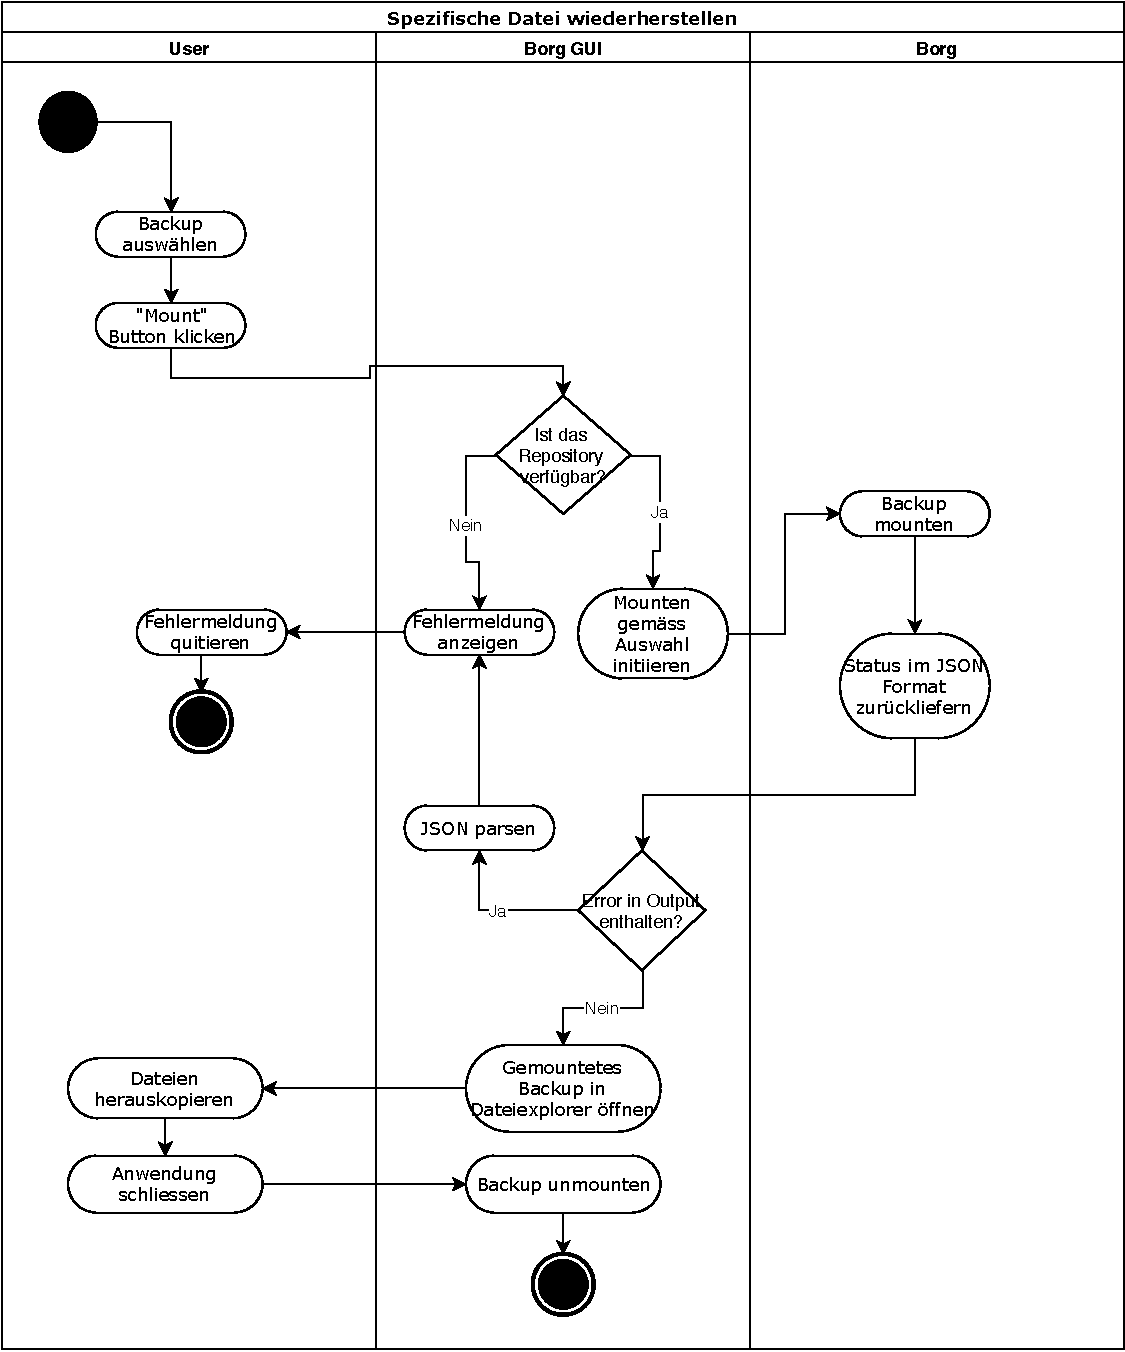
\includegraphics[width=.9\linewidth]{pictures/activity_mount.pdf}
\caption{\label{fig:org992f6bb}
Aktivitätsdiagramm für das spezifische Wiederherstellen einer Datei}
\end{figure}
\newpage
\paragraph{Use Case 4.1 Backup mounten}
\label{sec:orgae4ca85}

{\footnotesize
\begin{longtable}{|>{\columncolor[HTML]{EFEFEF}}p{.235\textwidth}|p{.7\textwidth}|}
\hline
\textbf{Identifier + Name} & 4.1 Backup mounten\\
\hline
\endfirsthead
\multicolumn{2}{l}{Fortsetzung von vorheriger Seite} \\
\hline

\textbf{Identifier + Name} & 4.1 Backup mounten \\

\hline
\endhead
\hline\multicolumn{2}{r}{Fortsetzung nächste Seite} \\
\endfoot
\endlastfoot
\hline
\textbf{Description} & Ein Backup wird als FUSE gemountet.\\
\hline
\textbf{Actors} & Borg GUI, \gls{borg}\\
\hline
\textbf{Status} & Freigegeben\\
\hline
\textbf{Includes} & -\\
\hline
\textbf{Trigger} & Das Borg GUI gibt an \gls{borg} den Input zum mounten weiter.\\
\hline
\textbf{Preconditions} & Use Case 1.0 wurde ausgeführt.\\
\hline
\textbf{Postconditions} & Das Backup wurde gemountet.\\
\hline
\textbf{Normal Flow} & 1. Borg GUI sammelt die Backup ID in Use Case 4.0.\\
 & 2. Borg GUI übergibt die Backup ID an \gls{borg} zusammen mit einem Zielpfad.\\
 & 3. \gls{borg} hängt das Backup als FUSE Laufwerk am Zielpfad ein.\\
 & 4. \gls{borg} meldet Erfolg an Borg GUI.\\
\hline
\textbf{Alternative Flow} & 1. Borg GUI sammelt die Backup ID in Use Case 4.0.\\
 & 2. Borg GUI übergibt die Backup ID an \gls{borg} zusammen mit einem Zielpfad.\\
 & 3. \gls{borg} hängt das Backup als FUSE Laufwerk am Zielpfad ein.\\
 & 4. \gls{borg} meldet einen Fehler an Borg GUI.\\
\hline
\textbf{Notes} & -\\
\hline
\textbf{UC History} & 1.0 Draft erstellt durch AZ\\
\hline
\textbf{Author} & A. Zweili\\
\hline
\textbf{Date} & 30.12.2018\\
\hline
\caption{\label{tab:orga3274db}
Use Case 4.1 Backup mounten}
\\
\end{longtable}
}

\newpage
\paragraph{Use Case 5.0 Konfiguration ändern}
\label{sec:org4e6f313}

{\footnotesize
\begin{longtable}{|>{\columncolor[HTML]{EFEFEF}}p{.235\textwidth}|p{.7\textwidth}|}
\hline
\textbf{Identifier + Name} & 5.0 Konfiguration ändern\\
\hline
\endfirsthead
\multicolumn{2}{l}{Fortsetzung von vorheriger Seite} \\
\hline

\textbf{Identifier + Name} & 5.0 Konfiguration ändern \\

\hline
\endhead
\hline\multicolumn{2}{r}{Fortsetzung nächste Seite} \\
\endfoot
\endlastfoot
\hline
\textbf{Description} & Das Verändern und Speichern der Konfiguration der Applikation.\\
\hline
\textbf{Actors} & User\\
\hline
\textbf{Status} & Freigegeben\\
\hline
\textbf{Includes} & -\\
\hline
\textbf{Trigger} & Ein User möchte die Einstellungen der Applikation anpassen.\\
\hline
\textbf{Preconditions} & Applikation gestartet.\\
\hline
\textbf{Postconditions} & -\\
\hline
\textbf{Normal Flow} & 1. Auf den Button "`Settings"' klicken.\\
 & 2. Ein neues Fenster mit den Einstellungen öffnet sich.\\
 & 3. Der Benutzer ändert mindestens eine Einstellung.\\
 & 4. Der Button "`OK"' wird angeklickt.\\
 & 5. Die Konfiguration wird in die Konfigurationsdatei geschrieben und in der Applikation geladen.\\
\hline
\textbf{Alternative Flow} & 1. Auf den Button "`Settings"' klicken.\\
 & 2. Ein neues Fenster mit den Einstellungen öffnet sich.\\
 & 3. Der Benutzer kann Einstellungen ändern.\\
 & 4. Der Button "`Cancel"' wird angeklickt.\\
 & 5. Jeglich Änderungen werden verworfen und die Konfigurationsdatei bleibt im aktuellen Zustand.\\
\hline
\textbf{Notes} & -\\
\hline
\textbf{UC History} & 1.0 Draft erstellt durch AZ\\
\hline
\textbf{Author} & A. Zweili\\
\hline
\textbf{Date} & 30.12.2018\\
\hline
\caption{\label{tab:org4ea078d}
Use Case 5.0 Konfiguration ändern}
\\
\end{longtable}
}

\begin{figure}[htbp]
\centering
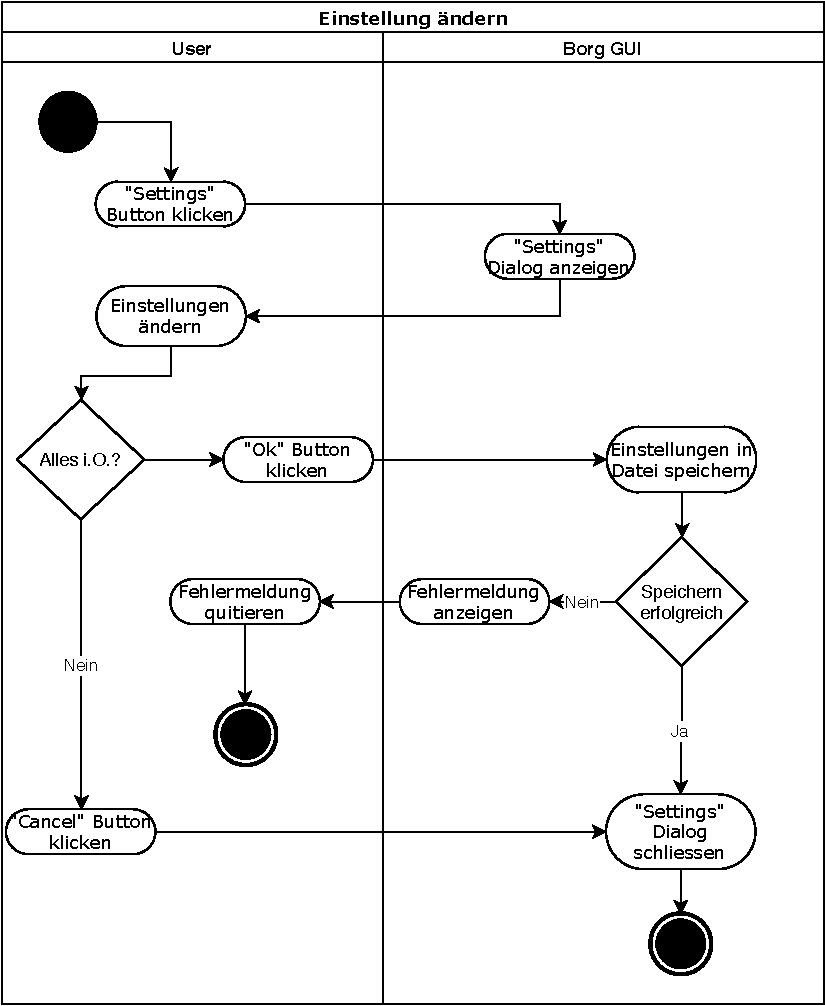
\includegraphics[width=.9\linewidth]{pictures/activity_settings.pdf}
\caption{\label{fig:org35467e2}
Aktivitätsdiagramm zum Ändern von Einstellungen}
\end{figure}
\newpage
\paragraph{Use Case 6.0 automatische Backups aktivieren}
\label{sec:org7ea0bf7}

{\footnotesize
\begin{longtable}{|>{\columncolor[HTML]{EFEFEF}}p{.235\textwidth}|p{.7\textwidth}|}
\hline
\textbf{Identifier + Name} & 6.0 automatische Backups aktivieren\\
\hline
\endfirsthead
\multicolumn{2}{l}{Fortsetzung von vorheriger Seite} \\
\hline

\textbf{Identifier + Name} & 6.0 automatische Backups aktivieren \\

\hline
\endhead
\hline\multicolumn{2}{r}{Fortsetzung nächste Seite} \\
\endfoot
\endlastfoot
\hline
\textbf{Description} & Ein Systemdienst wird hinterlegt zum ausführen automatischer Backups.\\
\hline
\textbf{Actors} & User\\
\hline
\textbf{Status} & Freigegeben\\
\hline
\textbf{Includes} & -\\
\hline
\textbf{Trigger} & Ein User möchte automatisierte Backups haben.\\
\hline
\textbf{Preconditions} & Eine funktionierende Konfiguration muss hinterlegt sein.\\
 & Applikation gestartet.\\
\hline
\textbf{Postconditions} & Ein Systemdienst wurde erstellt welcher jeden Tag ein Backup macht.\\
\hline
\textbf{Normal Flow} & 1. Auf den Button "`Settings"' klicken.\\
 & 2. Bei der Option "`Automatic Backups"' den Hacken setzen.\\
 & 3. Die Settings mit klick auf "`Ok"' schliessen und speichern.\\
\hline
\textbf{Alternative Flow} & 1. Auf den Button "`Settings"' klicken.\\
 & 2. Bei der Option "`Automatic Backups"' den Hacken setzen.\\
 & 3. Die Aktion mit klick auf "`Cancel"' abrechen.\\
\hline
\textbf{Notes} & -\\
\hline
\textbf{UC History} & 1.0 Draft erstellt durch AZ\\
\hline
\textbf{Author} & A. Zweili\\
\hline
\textbf{Date} & 30.12.2018\\
\hline
\caption{\label{tab:org3890696}
Use Case 6.0 automatische Backups aktivieren}
\\
\end{longtable}
}

\begin{figure}[htbp]
\centering
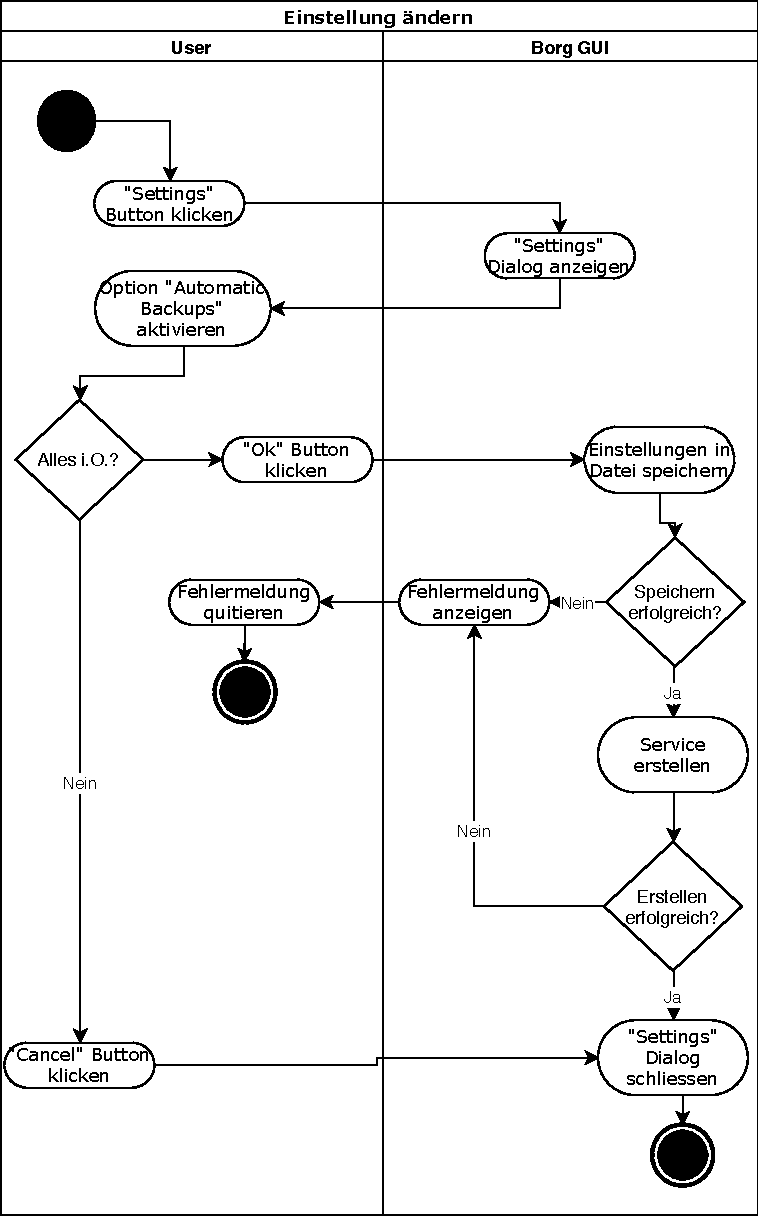
\includegraphics[width=.9\linewidth]{pictures/activity_automatic.pdf}
\caption{\label{fig:org839581b}
Aktivitätsdiagramm zum Aktivieren von automatischen Backups}
\end{figure}
\newpage
\section{Konzept}
\label{sec:orgd0ea4f6}

\subsection{Varianten}
\label{sec:org2b55ff8}

Da Borg eine JSON API zur Verfügung stellt bieten sich diverse Möglichkeiten um
das Programm anzubinden. Da das Ziel ist, das Programm normalen Nutzern
zugänglicher zu machen, bietet sich ein normales Desktop Programm am ehesten
an. Desktop Programme werden von allen Computer Usern täglich genutzt und sind
somit etwas was sie kennen.

Daraus ergeben sich die in diesem Kapitel aufgeführten Möglichkeiten für das
Projekt.

\subsubsection{Bewertung}
\label{sec:org34c4be3}

Die Bewertungspunkte setzen sich einerseits aus den Projektzielen anderseits
aus für das Projekt sinnvollen Punkten zusammen. Dadurch ergeben sich dann die
Bewertungen welche in der nachfolgenden Tabelle aufgenommen wurden. Die
möglichen Varianten wurden danach bewertet. Die effektive Berechnung des
Resultats wird nach folgender Formel durchgeführt.

\begin{equation}
G * EP = KE
\end{equation}

Also die Gewichtung(\emph{G}) multipliziert mit der erreichten Punktzahl(\emph{EP})
ergibt das Kriteriumsergebnis(\emph{KE}). Für das Endresultat wird dann die Summe
über alle Kriterien gebildet. Die Variante mit der höchsten Summe wurde für das
Projekt ausgewählt.

Mussziele erhalten dabei eine
Gewichtung von 10 und Wunschziele eine Gewichtung entsprechend der Bewertung in
der Tabelle Projektziele (\ref{tab:org9275be4}).

\begin{table}[htbp]
\centering
\begin{tabular}{|>{\columncolor[HTML]{EFEFEF}}p{4cm}|c|p{2cm}|p{2cm}|p{2cm}|}
\hline
\textbf{Kriterium}\cellcolor[HTML]{C0C0C0} & \textbf{Gewichtung}\cellcolor[HTML]{C0C0C0} & \textbf{max. Punktzahl}\cellcolor[HTML]{C0C0C0} & \textbf{erreichte Punktzahl}\cellcolor[HTML]{C0C0C0} & \textbf{Kriteriums- ergebnis}\cellcolor[HTML]{C0C0C0}\\
\hline
1. Cross Plattform nutzbar & 10 & 10 & 10 & 100\\
2. Freie Software & 5 & 10 & 10 & 50\\
3. Vorkenntnisse & 5 & 10 & 10 & 50\\
4. Integriert sich gut ins System & 5 & 10 & 10 & 50\\
5. Ohne spezielle Tools nutzbar & 5 & 10 & 10 & 50\\
6. Lesbarkeit des Codes & 5 & 5 & 5 & 25\\
7. Einfachheit des Setups & 5 & 5 & 5 & 25\\
8. Lernfaktor & 5 & 5 & 5 & 25\\
9. Verbreitung bei der BorgBackup Community & 5 & 5 & 5 & 25\\
10. Geschwindigkeit der Entwicklung & 3 & 5 & 5 & 15\\
\hline
\textbf{Total} &  &  &  & 415\\
\hline
\end{tabular}
\caption{\label{tab:org60d7038}
Muster Bewertungstabelle}

\end{table}

\subsubsection{Backend}
\label{sec:orgad0eeff}

Fürs Backend bieten sich die folgende drei Sprachen an: \hyperref[sec:org2369fca]{C\#}, \hyperref[sec:org5cb06df]{C++}, \hyperref[sec:org1e551c7]{Python}.
Dies vorallem weil alle Allrounder Sprachen sind und sich gut für Desktop
Applikationen eignen.

\paragraph{C\#}
\label{sec:org2369fca}

C\# ist eine von Microsoft entwickelte Programmiersprache welche viele
Frameworks zur Verfügung hat. Insbesondere Aufgrund der grossen kommerziellen
Nutzung und der guten Integration mit Windows hat C\# eine relative grosse
Verbreitung. Bei Linux und OS X ist es jedoch schwieriger C\# zu integrieren und
zu nutzen.

Sie ist zu Teilen \gls{libre}. Die Common Language Runtime welche für das
Ausführen von Software zuständig ist, ist unter der MIT Lizenz lizenziert
\footcite{csharp} der aktuelle Compiler Roslyn ist unter der Apache Lizenz
verfügbar \footcite{roslyn}. Da es sehr viele offiziele Teile um die Sprache C\#
gibt kann im Rahmen des Projektes nicht direkt abgeschätzt werden ob alle
benötigten Teile \gls{libre} sind. Für die Bewertung wird deshalb ein kleinerer
Wert als bei C++ und Python genommen.

C\# ist die Programmierspache welche an der IBZ hauptsächlich gelehrt wird.
Dadurch sind die Kenntnisse der Sprache und ihrer Anwendung bereits
einigermassen vorhanden. Ausserhalb der Schule wurde die Sprache jedoch noch nie
eingesetzt.

Entwickelt wird C\# hauptsächlich mit der \gls{ide} Microsoft Visual Studio.
Eine sehr umfangreiche und komlexe Software. Visual Studio ist dabei nur für
Windows und OS X erhältlich. Es ist auch möglich C\# Projekte ausserhalb von
Visual Studio zu erstellen ist jedoch nicht sehr einfach.

Der Code ist gut lesbar und es gibt offizielle Styleguides von Microsoft was
den Code über Projekte hinaus einigermassen einheitlich aussehen lässt. Zudem
hilft hier auch Visual Studio stark den Code entsprechend zu formatieren.
Besonders angenehm sind die Klassen- und Methodennamen der offiziellen
Frameworks. Insgesamt sehr gut gelöst aber in Sachen Lesbarkeit noch etwas
hinter Python.

Unter Windows ist das Setup von C\# relativ einfach. Allerdings ist es auch dort
im Vergleich zu Python eine umfangreiche Angelegenheit Visual Studio sauber zu
installieren und nutzbar zu machen. Auf anderen Plattform wird dies leider
nicht einfacher und unter Linux ist es bereits schwierig eine funktionierende
Umgebung in gang zu bringen.

Da C\# bereits an der IBZ gelernt wird ist der Lernfaktor hier im Vergleich zu
den anderen Sprachen sicher am kleinsten. Allerdings gibt es noch keinerlei
Kenntnisse beim Einbinden eines der unten aufgeführten \gls{gui} Frameworks.
Daher gibt es auf jeden Fall noch genügend zu lernen.

Die \gls{borg} Community hat vor relativ kurzer Zeit die offizielle Unterstützung
von Windows zurückgezogen. Da C\# eine sehr Windows lastige Sprache ist wird
daher davon ausgegangen das die Sprache innerhalb der \gls{borg} Community nicht
sehr verbreitet ist.

C\# ist eine stark typisiert Sprache und kompilierte Sprache. Desweiteren ist
Visual Studio der Erfahrung nach nicht die schnellste Software. Dies alles
führt dazu das C\# nicht gerade die schnellste Sprache zum programmmieren ist.
Jedoch aufgrund des moderneren Unterbaus sicher schneller als C++.

\begin{table}[htbp]
\centering
\begin{tabular}{|>{\columncolor[HTML]{EFEFEF}}p{4cm}|c|p{2cm}|p{2cm}|p{2cm}|}
\hline
\textbf{Kriterium}\cellcolor[HTML]{C0C0C0} & \textbf{Gewichtung}\cellcolor[HTML]{C0C0C0} & \textbf{max. Punktzahl}\cellcolor[HTML]{C0C0C0} & \textbf{erreichte Punktzahl}\cellcolor[HTML]{C0C0C0} & \textbf{Kriteriums- ergebnis}\cellcolor[HTML]{C0C0C0}\\
\hline
1. Cross Plattform nutzbar & 10 & 10 & 8 & 80\\
2. Freie Software & 5 & 10 & 8 & 40\\
3. Vorkenntnisse & 5 & 10 & 6 & 30\\
4. Integriert sich gut ins System & 5 & 10 & 8 & 40\\
5. Ohne spezielle Tools nutzbar & 5 & 10 & 6 & 30\\
6. Lesbarkeit des Codes & 5 & 5 & 4 & 20\\
7. Einfachheit des Setups & 5 & 5 & 2 & 10\\
8. Lernfaktor & 5 & 5 & 3 & 15\\
9. Verbreitung bei der BorgBackup Community & 5 & 5 & 1 & 5\\
10. Geschwindigkeit der Entwicklung & 3 & 5 & 3 & 9\\
\hline
\textbf{Total} &  &  &  & 279\\
\hline
\end{tabular}
\caption{\label{tab:orgc9c6090}
C\# Bewertungstabelle}

\end{table}

\paragraph{C++}
\label{sec:org5cb06df}

C++ ist eine stark typisierte und kompilierte Programmiersprache. Sie ist seit
1998 Teil des ISO Standards \footcite{cpp98}. ISO/IEC 14882:2017 \footcite{cpp17}
ist zur Zeit die aktuellste Variante. Die Sprache existiert seit ca. 33 Jahren
und hat eine weitreichende Verbreitung gefunden. C++ ist auf allen
Betriebssystemen gut unterstützt muss jedoch für jedes System separat
kompiliert werden.

Von C++ sind innerhalb des Projektes keinerlei Vorkenntnisse vorhanden. Dies
ist ein sehr hoher Risikofaktor.

C++ kompiliert direkt zu Maschinensprache und ist dadurch sehr performant und
läuft sehr gut auf jedem System. C++ ist im Vergleich zu modernen Sprachen
jedoch relativ komplex und bietet diverse Stolpersteine für Programmierer.

Zum entwickeln braucht es verhältnismässig wenig. Da die Sprache bereits sehr
alt ist, stammt sie noch aus einer Zeit wo man noch etwas rudimentärer
programmierte. Allerdings braucht man in jedem Fall einen \gls{compiler} um ein
ausführbares Programm zu erzeugen. Bei komplexeren Programmen wird man um
mindestens so etwas wie \glspl{makefile} auch nicht herumkommen.

Im Vergleich zu Python oder C\# ist C++ wohl die am schwersten lesbare Sprache.
Zudem gibt es auch keinen zentralen Styleguide welcher einem vorgeben würde wie
der Code am besten aussschauen sollte. Somit haben sich über die Jahre mehrere
Standards etabliert.

Der Lernfaktor wäre Aufgrund der mangelnden Vorkenntnisse hier ganz klar am
Grössten.

Da C++ eine alte Sprache ist geniesst sie auch eine dementsprechende
Verbreitung. Daher ist anzunehmen das sicher mindestens ein grössere Teil der
älteren BorgBackup Entwickler C++ oder C gelernt haben.

Da C++ auch heute noch zu den meistgenutzten Sprachen gehört gibt es
entsprechend viele Ressourcen dazu und Beispiel Projekte von denen man ableiten
kann. Auch hilfreiche Libraries gibts es sehr viele welche den Programmierer
unterstützen können. Die Sprache selber ist jedoch eher umständlich zu
schreiben. Hinzu kommt noch das man während der Entwicklung immer wieder den
Code kompilieren muss. In einem Projekt mit dieser begrenzten Zeitspanne eher
ungeeignet.

\begin{table}[htbp]
\centering
\begin{tabular}{|>{\columncolor[HTML]{EFEFEF}}p{4cm}|c|p{2cm}|p{2cm}|p{2cm}|}
\hline
\textbf{Kriterium}\cellcolor[HTML]{C0C0C0} & \textbf{Gewichtung}\cellcolor[HTML]{C0C0C0} & \textbf{max. Punktzahl}\cellcolor[HTML]{C0C0C0} & \textbf{erreichte Punktzahl}\cellcolor[HTML]{C0C0C0} & \textbf{Kriteriums- ergebnis}\cellcolor[HTML]{C0C0C0}\\
\hline
1. Cross Plattform nutzbar & 10 & 10 & 8 & 80\\
2. Freie Software & 5 & 10 & 10 & 50\\
3. Vorkenntnisse & 5 & 10 & 0 & 0\\
4. Integriert sich gut ins System & 5 & 10 & 8 & 40\\
5. Ohne spezielle Tools nutzbar & 5 & 10 & 6 & 30\\
6. Lesbarkeit des Codes & 5 & 5 & 2 & 10\\
7. Einfachheit des Setups & 5 & 5 & 3 & 15\\
8. Lernfaktor & 5 & 5 & 5 & 25\\
9. Verbreitung bei der BorgBackup Community & 5 & 5 & 3 & 15\\
10. Geschwindigkeit der Entwicklung & 3 & 5 & 2 & 6\\
\hline
\textbf{Total} &  &  &  & 271\\
\hline
\end{tabular}
\caption{\label{tab:orgba08048}
C++ Bewertungstabelle}

\end{table}

\paragraph{Python}
\label{sec:org1e551c7}

Der Python Interpreter ist für eine Vielzahl an Betriebssystemen erhältlich,
inklusive Windows, OS X und Linux. Nahezu jedes Desktop Linux System kommt mit
Python vor installiert. Auch OS X kommt bereits ab Werk mit Python Version 2.
Version 3 lässt sich sehr einfach nachinstallieren und ist einfach nutzbar.
Unter Windows geschtaltet sich die Installation etwas aufwändiger aber auch
nicht sehr kompliziert integriert sich in Windows jedoch etwas weniger elegant
als C\#.

Python ist freie Software unter der Python Software Foundation License
\footcite{python} und wird durch die Python Software Foundation in einem
Community basierten Modell entwickelt.

Die Vorkenntnisse sind im Vergleich zu C++ relativ gross und zu C\# etwas
weniger ausgeprägt. Es wurden damit im Rahmen der Ausbildung schon ein
grösseres Projekt realisiert und ansonsten mehrere kleine Projekte im Privaten
erstellen.

Für Python gibt es ein paar \glspl{ide} welchen den Programmierer bei seiner
Arbeit unterstützen können. Keine davon ist allerdings ein Muss um Python
programmieren zu können. Im einfachsten Fall wäre dies mit Notepad möglich. Ein
Editor mit etwas vortgeschritteren Features wäre jedoch empfehlenswert.

Python unterstützt mehrere Programmierungsparadigmen wie etwa
objekt-orientiert, funktionale oder Prozedurale Paradigmen. Bei der Entwicklung
von Python wurde sehr grossen Wert auf die Lesbarkeit der Sprache gelegt. Dies
mit dem Hintergedanken das eine Programmierspache viel häufiger gelesen als
effektiv geschrieben wird \footcite{pep8}.

Um ein Python Programm zu starten braucht es eigentlich kein grosses Setup.
Solange die Abhängigkeiten vorhanden sind, kann man ein Skript mit einem
einfachen Befehl, Code Snippet (\ref{org5e3d59f}) starten.

\lstset{language=bash,label=org5e3d59f,caption={Minimal Python Setup},captionpos=b,numbers=none}
\begin{sexylisting}{Minimal Python Setup}
python3 example.py
\end{sexylisting}

Da Python schon eine etwas bekanntere Sprache ist, ist der Lernfaktor der
Sprache selber nicht mehr so hoch. Allerdings gibt es noch viele interessante
Konzepte die man im Zusammenhang mit der Sprache lernen kann. Wie etwa zum
Beispiel multiple Vererbung von Klassen.

\gls{borg} selber wurde in Python geschrieben. Daher ist davon auszugehen das
Python innerhalb dieser Community eine sehr hohe Verbreitung geniesst.

Python ist eine dynamisch typisierte und interpretierte Sprache. Dies bedeutet
das man bei Variabeln nicht explizit den Typ angeben muss und die Programme zur
Laufzeit für den Computer übersetzt werden. Interpretierte Sprachen haben den
Vorteil das man mit ihnen in der Regel sehr schnell und unkompliziert
entwickeln kann, dies jedoch zu Lasten der Performance.

\begin{table}[htbp]
\centering
\begin{tabular}{|>{\columncolor[HTML]{EFEFEF}}p{4cm}|c|p{2cm}|p{2cm}|p{2cm}|}
\hline
\textbf{Kriterium}\cellcolor[HTML]{C0C0C0} & \textbf{Gewichtung}\cellcolor[HTML]{C0C0C0} & \textbf{max. Punktzahl}\cellcolor[HTML]{C0C0C0} & \textbf{erreichte Punktzahl}\cellcolor[HTML]{C0C0C0} & \textbf{Kriteriums- ergebnis}\cellcolor[HTML]{C0C0C0}\\
\hline
1. Cross Plattform nutzbar & 10 & 8 & 8 & 80\\
2. Freie Software & 5 & 10 & 10 & 50\\
3. Vorkenntnisse & 5 & 10 & 5 & 25\\
4. Integriert sich gut ins System & 5 & 10 & 8 & 40\\
5. Ohne spezielle Tools nutzbar & 5 & 10 & 7 & 35\\
6. Lesbarkeit des Codes & 5 & 5 & 4 & 20\\
7. Einfachheit des Setups & 5 & 5 & 4 & 20\\
8. Lernfaktor & 5 & 5 & 3 & 15\\
9. Verbreitung in der BorgBackup Community & 5 & 5 & 5 & 25\\
10. Geschwindigkeit der Entwicklung & 3 & 5 & 4 & 12\\
\hline
\textbf{Total} &  &  &  & 322\\
\hline
\end{tabular}
\caption{\label{tab:orga748a93}
Python Bewertungstabelle}

\end{table}

\subsubsection{FrontEnd}
\label{sec:org3ea116b}

Fürs Frontend sind folgende Projekte interessant: \hyperref[sec:orgb9798d9]{Qt}, \hyperref[sec:orge4f95de]{Gtk} und \hyperref[sec:orgf2a5cfb]{Electron}. Alle
drei sind cross-plattfrom fähige \gls{gui} Frameworks und nicht von einer
spezifischen Sprache abhängig. Da nahezu keine Erfahrung mit den aufgeführten
Frameworks vorhanden ist werden bei den Frontenend Frameworks die Punkte der
Verbreitung in der Community und Geschwindigkeit der Entwicklung ausgeschlossen
da in allen Fällen nicht mal eine ungenaune Schätzung wirklich möglich wäre.

\paragraph{Qt}
\label{sec:orgb9798d9}

Qt \footcite{qt}, "`cute"' ausgesprochen, ist ein Framework zum Entwickeln von
grafischen Oberflächen welche auf verschiedenen System ohne grosse Änderungen
laufen sollen und sich dabei soweit als möglich wie eine native Applikation
verhalten und "`anfühlen"' soll.

Die Rechte an Qt hält die Firma "`The Qt Company"'. Das Framework Qt wird jedoch
offen entwickelt und die Community hat ein Mitspracherecht. Die Linux
Desktopumgebung KDE nutzt das Qt Framework intensiv. Qt ist \gls{libre} und der
\gls{gpl} v3 \footcite{qtlicense} oder mit einer kostenpflichtigen proprietären
Lizen erhältlich falls die \gls{gpl} nicht genutzt werden kann.

Vorkenntnisse zu Qt sind nur sehr wenig vorhanden. Mehr als ein paar Tests
wurden damit noch nicht gemacht.

Eine Qt Oberfläche kann direkt in der jeweiligen Sprache des Backends
geschrieben werden oder Mittels des Qt Designers als XML Datei gespeichert und
dann in die eigentliche Applikation importiert werden. Somit ist keine
spezielle Software nötig.

XML ist nicht übermässig gut lesbar allerdings kann man Qt in der verwendeten
Sprache programmiert werden somit ist es hauptsächlich von der Sprache im
Backend abhängig. Die Dokumentation ist in C++ geschrieben was für einen
Entwickler ohne C++ Kenntnisse die Software etwas unzugänglich macht.

Qt scheint, soweit dies bis jetzt abgeschätzt werden kann, sehr leicht in ein
Projekt zu integrieren sein.

Da noch sehr wenig Kenntnisse vorhanden sind ist der Lernfaktor entsprechend
gross.

\begin{table}[htbp]
\centering
\begin{tabular}{|>{\columncolor[HTML]{EFEFEF}}p{4cm}|c|p{2cm}|p{2cm}|p{2cm}|}
\hline
\textbf{Kriterium}\cellcolor[HTML]{C0C0C0} & \textbf{Gewichtung}\cellcolor[HTML]{C0C0C0} & \textbf{max. Punktzahl}\cellcolor[HTML]{C0C0C0} & \textbf{erreichte Punktzahl}\cellcolor[HTML]{C0C0C0} & \textbf{Kriteriums- ergebnis}\cellcolor[HTML]{C0C0C0}\\
\hline
1. Cross Plattform nutzbar & 10 & 10 & 10 & 100\\
2. Freie Software & 5 & 10 & 10 & 50\\
3. Vorkenntnisse & 5 & 10 & 2 & 10\\
4. Integriert sich gut ins System & 5 & 10 & 8 & 40\\
5. Ohne spezielle Tools nutzbar & 5 & 10 & 8 & 40\\
6. Lesbarkeit des Codes & 5 & 5 & 3 & 15\\
7. Einfachheit des Setups & 5 & 5 & 4 & 20\\
8. Lernfaktor & 5 & 5 & 4 & 20\\
\hline
\textbf{Total} &  &  &  & 295\\
\hline
\end{tabular}
\caption{\label{tab:org8d19685}
Qt Bewertungstabelle}

\end{table}

\paragraph{Gtk}
\label{sec:orge4f95de}

Gtk ist sowohl für Linux wie auch für Windows und OS X erhältlich. Gtk hat als
Projekt der Gnome Foundation seine Wurzeln jedoch ganz klar in der Linux Welt.
Gtk ist \gls{libre} under der Lesser General Public Lizenz \footcite{gtklicense}.
Gtk ist ein Projekt der GNOME Foundation einer nicht für Profit Organisation
welche die Entwicklung diverser freier Software Projekte koordiniert.

Zu Gtk gibt es keinerlei Vorkenntnisse als Programmierer. Gtk wurde bis jetzt
nur intensiv User verwendet.

Gtk integriert sich nur unter Linux wirklich gut ins System. Unter Windows und
OS X können die Applikation schnell etwas fremd wirken. Dies ist gut bei der
Applikation Meld \footcite{meld} zu sehen wenn man eine Datei auswählen möchte,
Abbildung (\ref{fig:orgeedd70e}).

\begin{figure}[htbp]
\centering
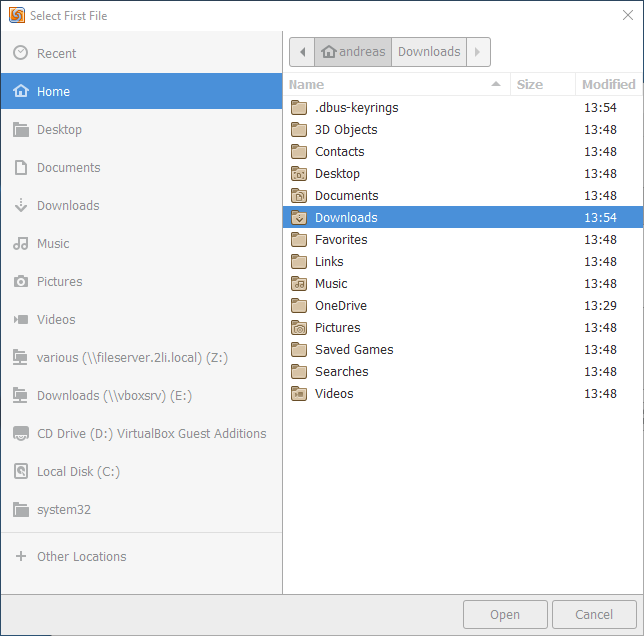
\includegraphics[width=.9\linewidth]{pictures/meld.png}
\caption{\label{fig:orgeedd70e}
Screenshot der Applikation Meld unter Windows 10}
\end{figure}
Die Gtk Dokumentation empfiehlt \footcite{gtk_setup}, das man unter Windows das
Programm MSYS2 installiert um Gtk einzurichten. Zum Programmieren an sich
braucht es offenbar nicht zwingend weitere Tools aus einem Editor. Wie auch bei
Qt hat man jedoch die Möglichkeit das \gls{gui} mit einem \gls{gui} Designer
grafisch zu erstellen.

Wie auch Qt kann man Gtk entweder direkt in der Backend Sprach programmieren
oder aus dem \gls{gui} Designer dann als XML exportieren. Der Code in der
Dokumentation ist in C geschrieben was auch nicht die zugängliste Sprache ist.

Die Verwendung von Gtk innerhalb des Programms scheint ähnlich einfach zu sein
wie bei Qt. Die Installation ist allerdings unter Windows eher das Gegenteil
von einfach.

Da die Kenntnisse gleich null sind ist der Lernfaktor auf dem Maximum.

\begin{table}[htbp]
\centering
\begin{tabular}{|>{\columncolor[HTML]{EFEFEF}}p{4cm}|c|p{2cm}|p{2cm}|p{2cm}|}
\hline
\textbf{Kriterium}\cellcolor[HTML]{C0C0C0} & \textbf{Gewichtung}\cellcolor[HTML]{C0C0C0} & \textbf{max. Punktzahl}\cellcolor[HTML]{C0C0C0} & \textbf{erreichte Punktzahl}\cellcolor[HTML]{C0C0C0} & \textbf{Kriteriums- ergebnis}\cellcolor[HTML]{C0C0C0}\\
\hline
1. Cross Plattform nutzbar & 10 & 10 & 10 & 100\\
2. Freie Software & 5 & 10 & 10 & 50\\
3. Vorkenntnisse & 5 & 10 & 0 & 0\\
4. Integriert sich gut ins System & 5 & 10 & 6 & 30\\
5. Ohne spezielle Tools nutzbar & 5 & 10 & 8 & 40\\
6. Lesbarkeit des Codes & 5 & 5 & 3 & 15\\
7. Einfachheit des Setups & 5 & 5 & 3 & 15\\
8. Lernfaktor & 5 & 5 & 5 & 25\\
\hline
\textbf{Total} &  &  &  & 275\\
\hline
\end{tabular}
\caption{\label{tab:org8321157}
Gtk Bewertungstabelle}

\end{table}

\paragraph{Electron}
\label{sec:orgf2a5cfb}

Electron ist ein cross-platform Framework zum entwickeln von \glspl{gui} welches
dabei jedoch auf Technologien aus der Webentwicklung benutzt. Entwickelt wird
Electron von der Firma Github und ist \gls{libre} unter der MIT Lizenz
\footcite{electronlicense}.

Da Electron auf Technologien aus der Webentwicklung setzt sind hier im
Vergleich bereit gute Kenntnisse vorhanden. Über die genau Funktion und
Implementierung sind noch keine Kenntnisse vorhanden.

Die Verwendung von Webtechnologien macht Electron zwar sehr kompatibel auf den
unterstützten Systemen, oftmals sehen die Applikationen jedoch doch eher wie
eine Webseite als wie eine Desktop Applikation aus. Ein weitere Nachteil ist
der hohe Ressourcenverbrauch da jede Applikation nahezu einer eigenene Instanz
des Google Chrome Browsers gleich kommt.

Bei der Installation muss Nodejs und der Paket Manager von Nodejs, NPM,
vorhanden sein. Zum Programmieren selber braucht es keine speziellen Tools. Ein
Editor und ein Webbrowser sollten aussreichend sein.

Electron Applikationen bestehen hauptsächlich aus HTML, CSS und JavaScript
Code. Wenn man nich die komplette Applikation in NodeJS programmieren möchte
kommt dann noch eine zusätzliche Sprache hinzu. HTML ist ähnlich müsahm zu
lesen wie XML. CSS und JavaScript sind relativ angenehm zu lesen wobei es für
beide keine offiziellen Style Guides gibt. Was bei Webanwendungen jedoch immer
das schwierigste ist, ist der wechsel zwischen verschiedenen Sprachen und
Konzepten. Dieses Problem hat man bei Electron leider auch.

Das Setup von Electron ist etwa ähnlich kompliziert wie das Setup von Gtk und
ist sehr ähnlich dem Entwickeln einer normalen Webapplikation.

Da an der IBZ Webtechnologien bereits intensiv behandelt worden sind und man in
diesem Rahmen bereits ein paar Webapplikationen erstellt hat wäre der
Lernfaktor bei Electron wohl nicht so gross wie etwa bei Qt oder Gtk.

\begin{table}[htbp]
\centering
\begin{tabular}{|>{\columncolor[HTML]{EFEFEF}}p{4cm}|c|p{2cm}|p{2cm}|p{2cm}|}
\hline
\textbf{Kriterium}\cellcolor[HTML]{C0C0C0} & \textbf{Gewichtung}\cellcolor[HTML]{C0C0C0} & \textbf{max. Punktzahl}\cellcolor[HTML]{C0C0C0} & \textbf{erreichte Punktzahl}\cellcolor[HTML]{C0C0C0} & \textbf{Kriteriums- ergebnis}\cellcolor[HTML]{C0C0C0}\\
\hline
1. Cross Plattform nutzbar & 10 & 10 & 10 & 100\\
2. Freie Software & 5 & 10 & 10 & 50\\
3. Vorkenntnisse & 5 & 10 & 5 & 25\\
4. Integriert sich gut ins System & 5 & 10 & 4 & 20\\
5. Ohne spezielle Tools nutzbar & 5 & 10 & 7 & 35\\
6. Lesbarkeit des Codes & 5 & 5 & 3 & 15\\
7. Einfachheit des Setups & 5 & 5 & 3 & 15\\
8. Lernfaktor & 5 & 5 & 3 & 15\\
\hline
\textbf{Total} &  &  &  & 275\\
\hline
\end{tabular}
\caption{\label{tab:org6e61af0}
Electron Bewertungstabelle}

\end{table}

\subsubsection{Ergebnis}
\label{sec:orgb914223}

Aufgrund der erreichten Punktzahl, Tabelle:(\ref{tab:org609b05e}), bei den vorhergehenden
Variantenbewertungen, wurde entschieden für das Backend der Applikation auf
Python zu setzen und fürs Frontend Qt zu benutzen.
\begin{table}[H]
\centering
\begin{tabular}{|>{\columncolor[HTML]{EFEFEF}}p{4.5cm}|r|}
\hline
\textbf{Variante}\cellcolor[HTML]{C0C0C0} & \textbf{Erreichte Punktzahl}\cellcolor[HTML]{C0C0C0}\\
\hline
\textbf{Backend} & \\
C\# & 279\\
C++ & 271\\
Python & 322\\
\textbf{Frontend} & \\
Qt & 295\\
Gtk & 275\\
Electron & 275\\
\hline
\end{tabular}
\caption{\label{tab:org609b05e}
Variantenbewertung Ergebnis}

\end{table}

\subsection{Vorkenntnisse}
\label{sec:org4ef797a}

Die benötigten Vorkenntnisse wurden in den vorangegangenen Semestern erarbeitet
und sind in der Basis gefestigt. Erfahrungen im Bereich der Entwicklung von
Desktop Applikationen sind zum Teil vorhanden. Jedoch hauptsächlich für Windows
Systeme und C\#.

\subsection{Testing}
\label{sec:org4efee39}

PLACEHOLDER

\subsubsection{Testfälle}
\label{sec:org55477bd}

PLACEHOLDER

\section{Realisierung}
\label{sec:org084b9b2}
\subsection{Cross-plattform Kompatibilität}
\label{sec:orgc58cfd4}

Um sicherzugehen das die gewählten Technologien auch den Anforderungen
entsprechen wurde ein kleines "`Hello World"' Programm mit Python3 und Qt
geschrieben. Dieses läuft ohne jegliche Probleme und Anpassung auf Windows,
Linux und OS X. Wie in den Screenshots in Abbildung:(\ref{fig:org0701830}) zu sehen
ist.

\begin{figure}[htbp]
\centering
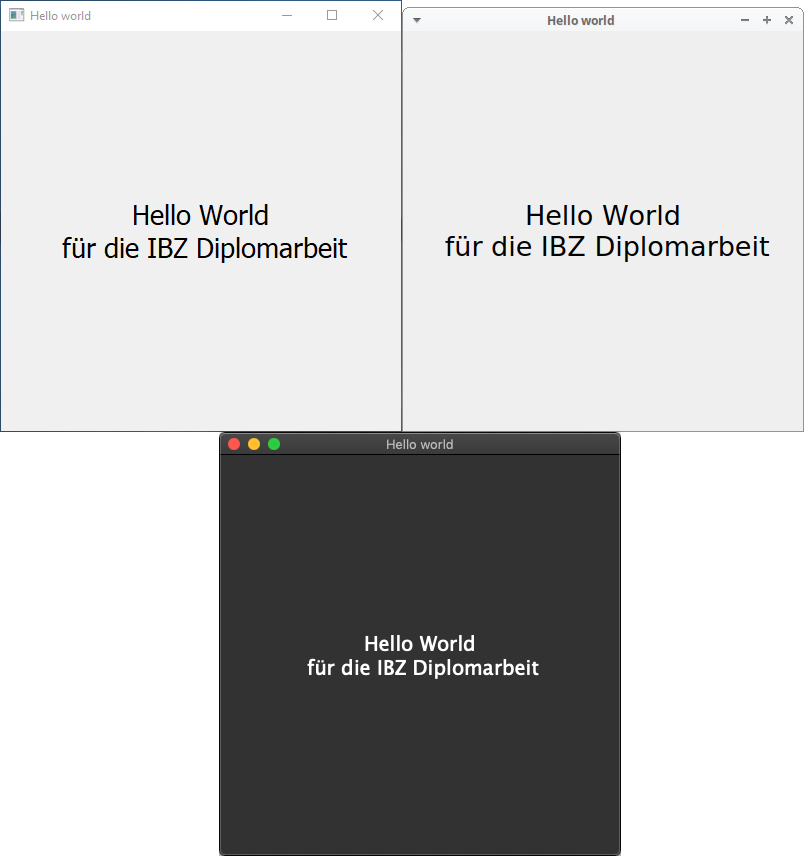
\includegraphics[width=.9\linewidth]{pictures/hello_world.png}
\caption{\label{fig:org0701830}
Python und Qt Applikation unter Windows (links), Linux (rechts) und OS X (unten)}
\end{figure}

\subsection{Benutzerinterface}
\label{sec:org50839f2}
\paragraph{Inspiration}
\label{sec:org1cb94b4}

PLACEHOLDER

\paragraph{Frontend Umsetzung}
\label{sec:org355e7a6}

PLACEHOLDER

\paragraph{Backend Umsetzung}
\label{sec:org263b030}

PLACEHOLDER

\section{Ausblick}
\label{sec:org4832c62}
\subsection{Projektmanagement}
\label{sec:org1794ec5}

PLACEHOLDER

\subsection{Umsetzung}
\label{sec:org1ca9bef}

PLACEHOLDER

\subsection{Gelerntes}
\label{sec:orgd179673}

PLACEHOLDER

\newpage
\begin{landscape}
\section{Arbeitsjournal}
\label{sec:orgf31d4c9}

\begin{longtable}{|p{2cm}|p{5cm}|p{5cm}|p{7cm}|}
\hline
\textbf{Datum}\cellcolor[HTML]{C0C0C0} & \textbf{Geplante Arbeiten}\cellcolor[HTML]{C0C0C0} & \textbf{Erreichte Arbeiten}\cellcolor[HTML]{C0C0C0} & \textbf{Eindruck}\cellcolor[HTML]{C0C0C0}\\
\hline
\endfirsthead
\multicolumn{4}{l}{Fortsetzung von vorheriger Seite} \\
\hline

\textbf{Datum}\cellcolor[HTML]{C0C0C0} & \textbf{Geplante Arbeiten}\cellcolor[HTML]{C0C0C0} & \textbf{Erreichte Arbeiten}\cellcolor[HTML]{C0C0C0} & \textbf{Eindruck}\cellcolor[HTML]{C0C0C0} \\

\hline
\endhead
\hline\multicolumn{4}{r}{Fortsetzung nächste Seite} \\
\endfoot
\endlastfoot
\hline
16.12.2018 & Zeitplan erarbeiten, Ziele dokumentieren & keine Abweichung & -\\
\hline
23.12.2018 & Lösungsvarianten erfassen, Lösungsvarianten bewerten, Lösungsvariante bestimmen, SWOT Analyse erstellen, 1. Meeting & keine Abweichung & Marco Frei hat noch diverse Punkte eingebracht die, die Planung ziemlich durcheinander bringen. Bedeute viel zusätzliche Arbeit.\\
\hline
30.12.2018 & Controlling erarbeiten, Ist- und Soll-Analyse, SWOT Analyse, Umweltanalyse, Massnahmen Katalog erarbeiten, User Stories erarbeiten, Use Case Diagramm erstellen, Use Cases ausarbeiten, Anforderungskatalog erstellen, UML Diagramme & keine Abweichung & UML Diagramme für eine Software zu erstellen die nicht existiert ist noch eine interessante Herausforderung.\\
\hline
06.01.2019 & Lösungsvarianten erarbeiten und entscheiden, Test Konzept beschreiben und Testfälle erstellen &  & \\
\hline
\caption{\label{tab:org109e680}
Arbeitsjournal}
\\
\end{longtable}
\end{landscape}
